% --------------------------------------------------------------------

\chapter[Some Example Observing Strategies]{Some Example Observing Strategies}
\def\chpname{cadexp}\label{chp:\chpname}

\credit{ivezic}
\noindent {\it
and the LSST Simulations Team, LSST Project Science Team, and Others
}

% --------------------------------------------------------------------

\noindent{\bf Summary:} In this chapter (which was originally prepared
as the standalone report available from
\url{http://www.astro.washington.edu/users/ivezic/lsst/cadexp2.pdf})
we analyze and compare the performance of a number of simulated LSST
observing strategies (``cadences'')
which were developed in support of the LSST 2015 Observing
Strategy Workshop.  A candidate new Baseline Cadence,
\opsimdbref{db:enigma}, was found adequate and is proposed as  a
replacement for the previous Baseline Cadence (\texttt{opsim3.61}).
Simulations that only implemented Universal
Cadence proposal imply a margin of about 40\% relative to the design
specifications for the main survey sky coverage and the number of
visits per field from the Science Requirements Document. This margin
can be used to increase the sky coverage of the main survey, the total
number of visits per field, or to implement special programs, such as
deep drilling fields and Galactic plane coverage. Several  simulations
analyzed here quantitatively explore these strategic options.
Additional simulations show that the effects of variations of the
visit exposure time in the  range 20-60 seconds on surveying
efficiency can be predicted using simple efficiency estimates. Various
modifications of baseline cadence (e.g. Pan-STARRS-like cadence,  no
visit pairs, sequences with 3 and 4 visits) indicate a large parameter
space for further optimization, especially for time-domain
investigations and detailed coverage of special sky regions.

% --------------------------------------------------------------------

\section{Introduction}
\def\secname{cadexp:intro}\label{sec:\secname}

With the release of the latest version of Operations Simulations
(hereafter \OpSim) code (version 3.2.1)  for simulating LSST
deployment, and the active development of Metrics Analysis Framework
(\MAF,  currently version 0.2) for analyzing \OpSim outputs, we can
now begin to undertake systematic and  massive investigations of
various LSST deployment strategies.

The optimization of the ultimate LSST observing strategy will be done
with significant input from  the community. To facilitate this
process, the first of a series of meetings, named ``LSST \& NOAO
Observing Cadences Workshop'', was held during the
\href{https://project.lsst.org/meetings/ocw}{LSST 2014 meeting} in
Phoenix, AZ, August 11-15, 2014. The next workshop , named ``LSST
Observing Strategy Workshop'',  will be held
\href{http://lsstsciencecollaborations.github.io/ObservingStrategy/}{after
the LSST 2015 meeting} in Bremerton, WA, August 20-22, 2015.

In part as a preparation for this upcoming workshop, the LSST
Simulations Team and the Project Science Team have designed, executed
and analyzed a number of simulated surveys.  The cadence strategies
for these surveys, while similar to Baseline Cadence, are modified to
study the impact of various strategy variations on the scientific
potential of LSST. The cadence set also includes a candidate baseline
cadence replacement.

An initial analysis of these simulated surveys is presented here.
\href{https://confluence.lsstcorp.org/display/SIM/MAF+documentation}{MAF}
reports for all simulated cadences are available from \begin{verbatim}
http://tusken.astro.washington.edu:8080/?runId=2 \end{verbatim}

\listofopsimdbs

\navigationbar

% --------------------------------------------------------------------

\section{The Baseline Observing Strategy}
\def\secname{cadexp:baseline}\label{sec:\secname}

The current ``official'' (managed by the LSST Change Control Board)
Baseline Cadence, \texttt{opsim3.61},  was produced with an old version of
\OpSim code. We first introduce a candidate replacement simulation
that was produced using  the latest version (v3.2.1) of \OpSim code,
and then proceed with the analysis of other simulations that modify
observing strategy in various informative ways. Suggestions for
further tool development, and a summary of the main cadence questions
addressed  here are available at end of this document.

% - - - - - - - - - - - - - - - - - - - - - - - - - - - - - - - - - -

%%%%%%%%%%%%%%%%%%%%%%%%%%%%%%%%%
\opsimdb[db:enigma]{enigma\_1189}{the new Baseline Cadence.}
%%%%%%%%%%%%%%%%%%%%%%%%%%%%%%%%%

%%%%%%%%%%%%%%%%%%%%%%%%%%%%%%%%%
\begin{figure}[tbh!]
\vskip -1.3in
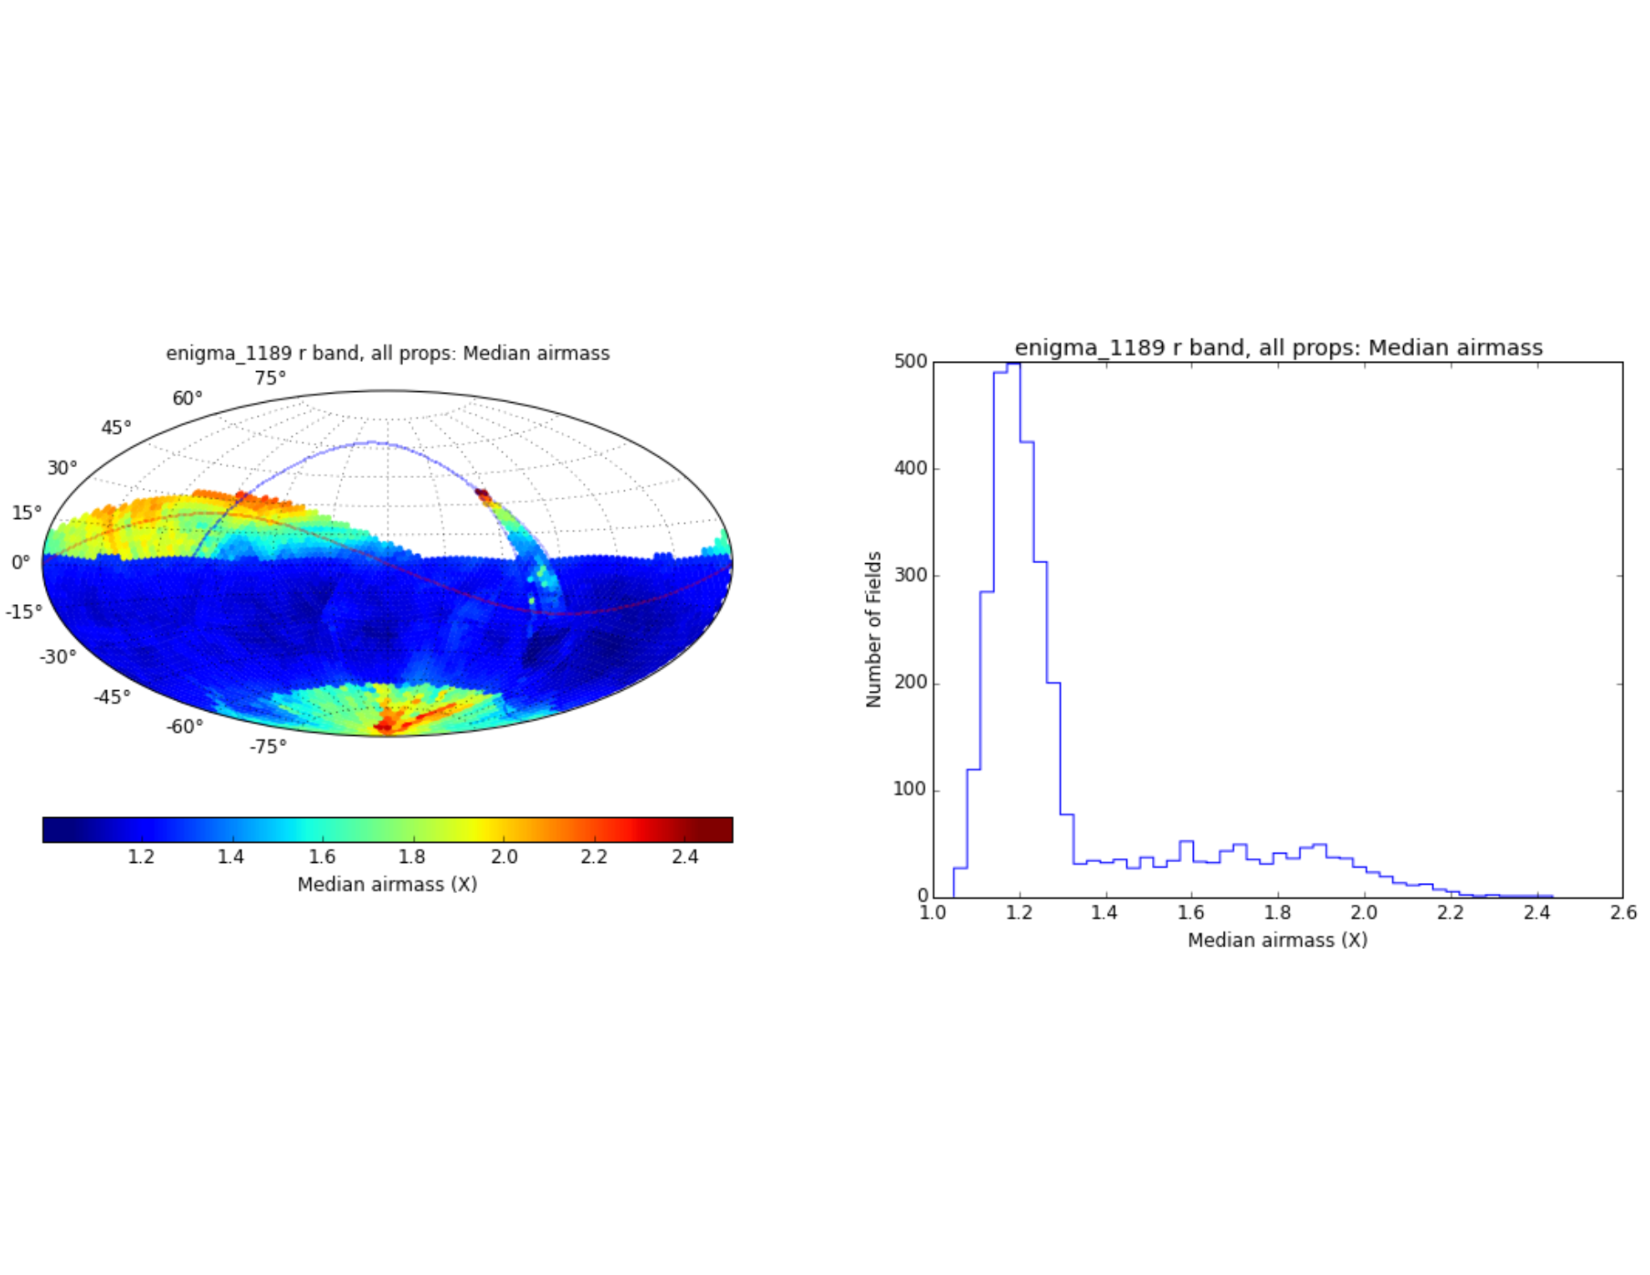
\includegraphics[angle=0,width=0.99\hsize:,clip]{figs/enigma1189_airmass.pdf}
\vskip -1.3in
\caption{The median airmass in the $r$ band across the sky for simulated cadence
\opsimdbref{db:enigma} is shown in Aitoff
projection of equatorial coordinates in the left panel. The corresponding histogram is
shown in the right panel. For the main survey area, the maximum allowed airmass
was set to 1.5. }
\label{fig:airmassenigma}
\end{figure}
%%%%%%%%%%%%%%%%%%%%%%%%%%%%%%%%%

%%%%%%%%%%%%%%%%%%%%%%%%%%%%%%%%%
\begin{figure}[t!]
\vskip -0.1in
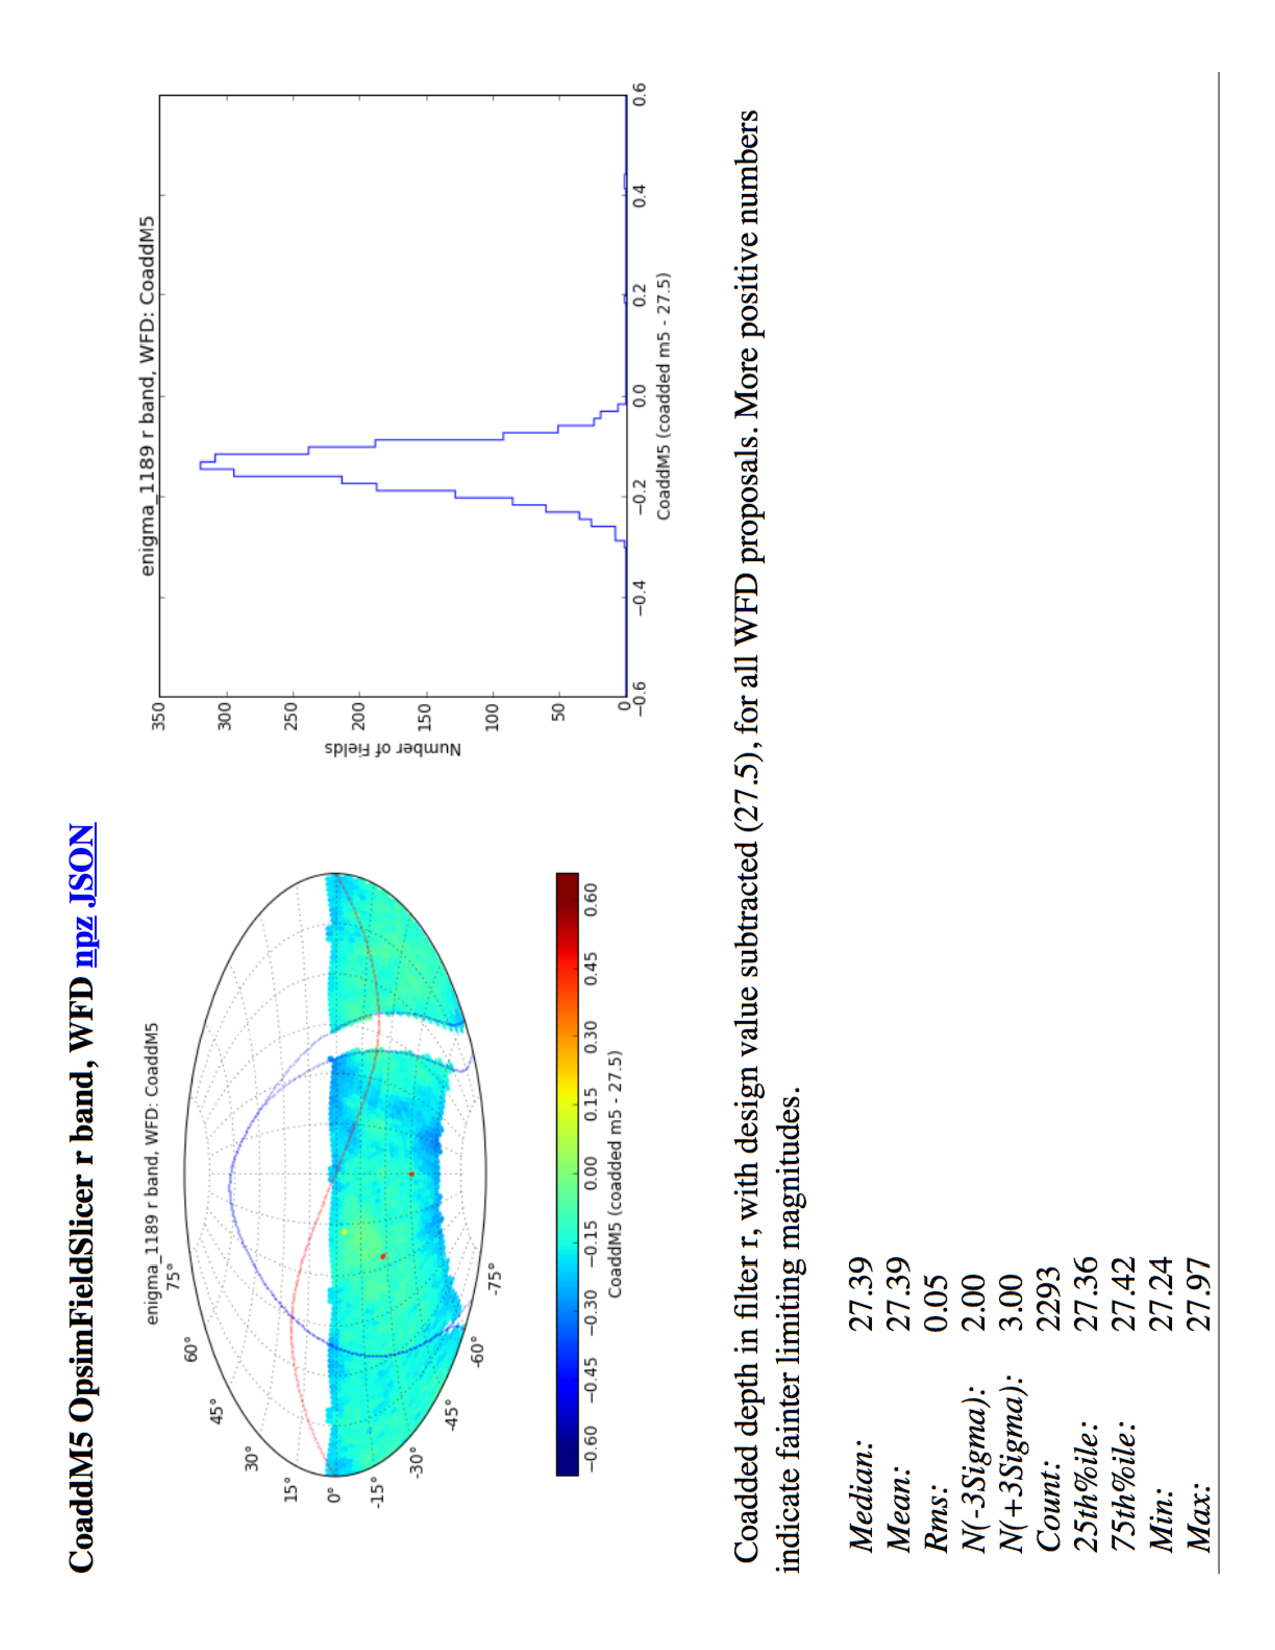
\includegraphics[angle=270,width=0.99\hsize:,clip]{figs/enigma1189_DWFcoaddr5.pdf}
\caption{A screen grab from web-based MAF analysis of simulated cadence
\opsimdbref{db:enigma}. The coadded $5\sigma$ depth for point sources in the $r$ band
across the main survey area (WFD=``wide-fast-deep'') is shown in the top left corner,
in Aitoff projection of equatorial coordinates. The red line shows the Ecliptic and
the blue line shows the Galactic equator (it bifurcates around the so-called
``Galactic confusion zone'').  The distribution of the limiting depth across this
area is shown as a histogram in the top right corner. The basic statistics for
this distribution are listed in the bottom left.}
\label{fig:coaddm5enigma}
\end{figure}
%%%%%%%%%%%%%%%%%%%%%%%%%%%%%%%%%

%%%%%%%%%%%%%%%%%%%%%%%%%%%%%%%%%
\begin{figure}[t!]
\vskip -0.0in
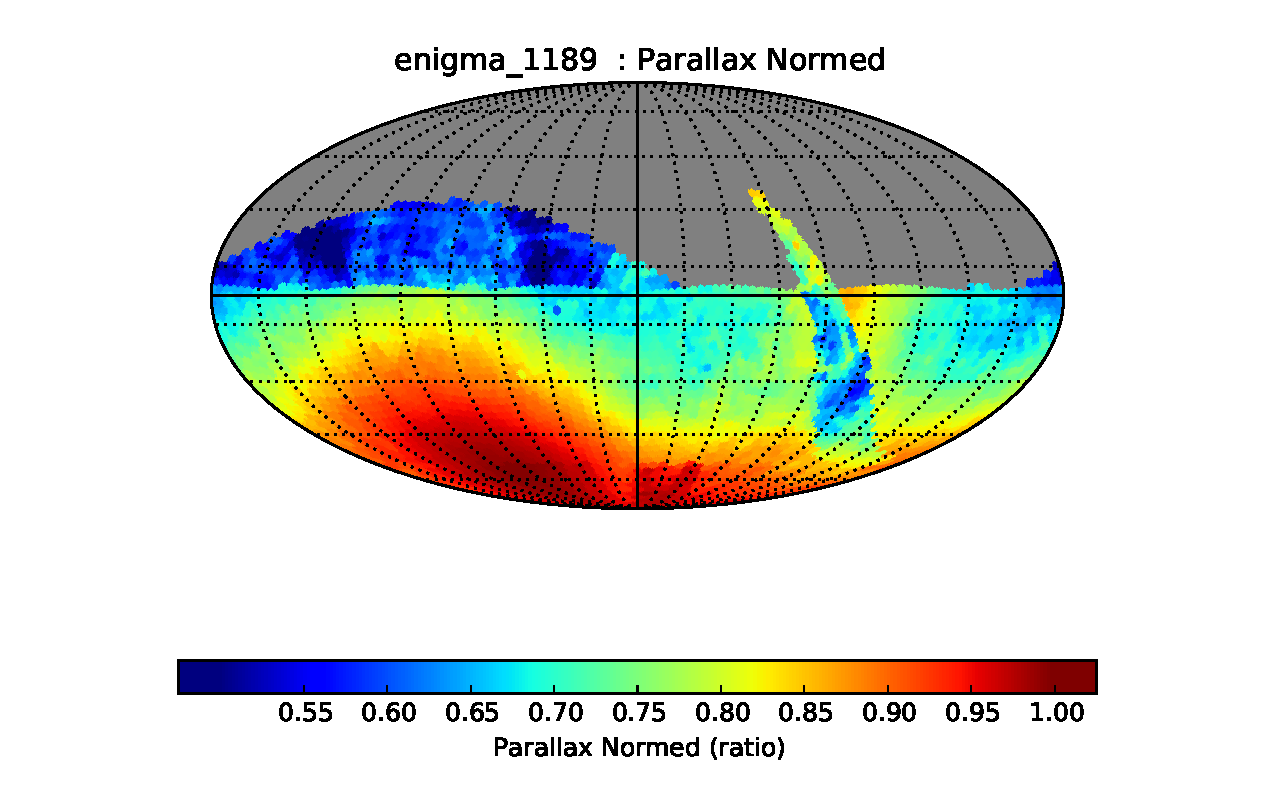
\includegraphics[angle=0,width=0.49\hsize:,clip]{figs/enigma_1189_Parallax_Normed__HEAL_SkyMap.pdf}
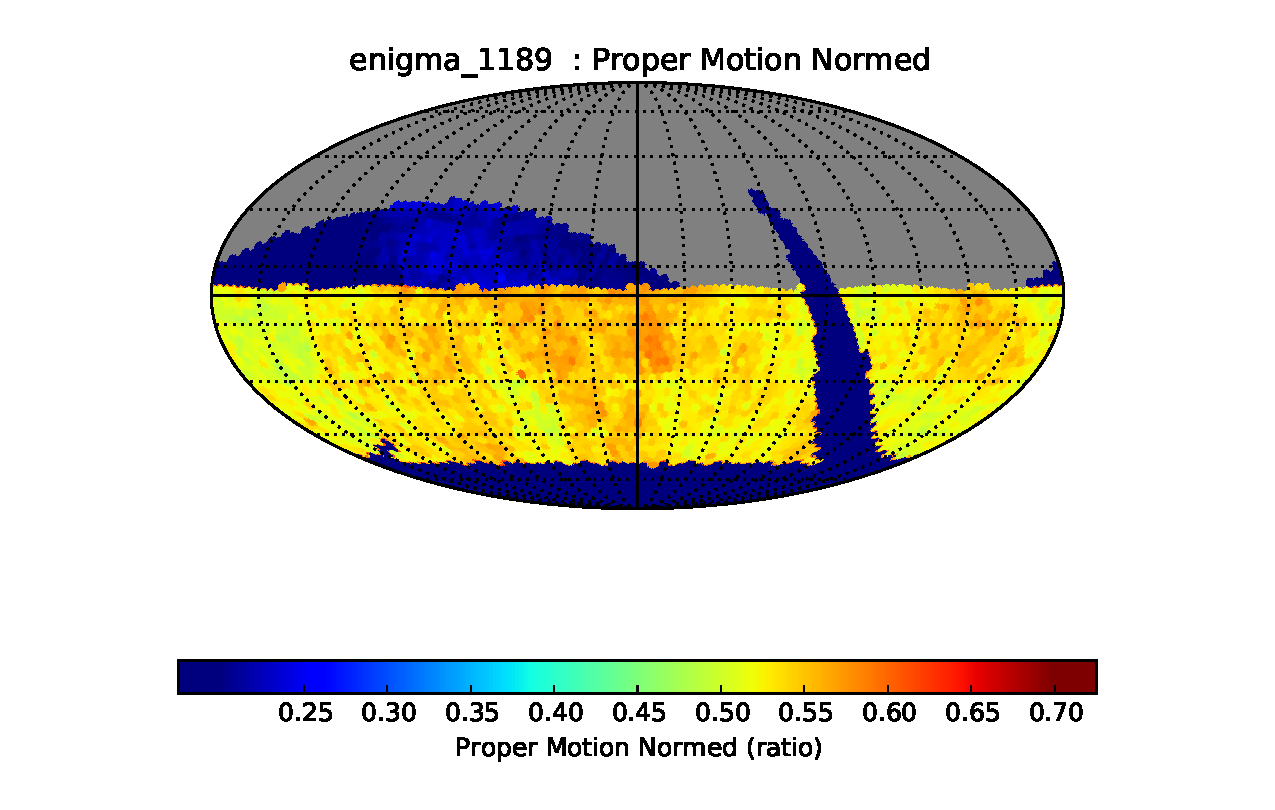
\includegraphics[angle=0,width=0.49\hsize:,clip]{figs/enigma_1189_Proper_Motion_Normed__HEAL_SkyMap.pdf}
\vskip -0.1in
\caption{The trigonometric parallax errors (left) and proper motion errors (right), normalized
by the values for idealized perfectly optimized cadences (parallax: all the observations are taken
at maximum parallax factor, resulting in a peak at the South Ecliptic pole; proper motion:
a half of all visits are obtained on the first day and the rest on the last day of the survey),
obtained for simulated cadence \opsimdbref{db:enigma} are shown in Aitoff projection of equatorial
coordinates.}
\label{fig:parapmenigma}
\end{figure}
%%%%%%%%%%%%%%%%%%%%%%%%%%%%%%%%%

%%%%%%%%%%%%%%%%%%%%%%%%%%%%%%%%%
\begin{figure}[t!]
\vskip -0.2in
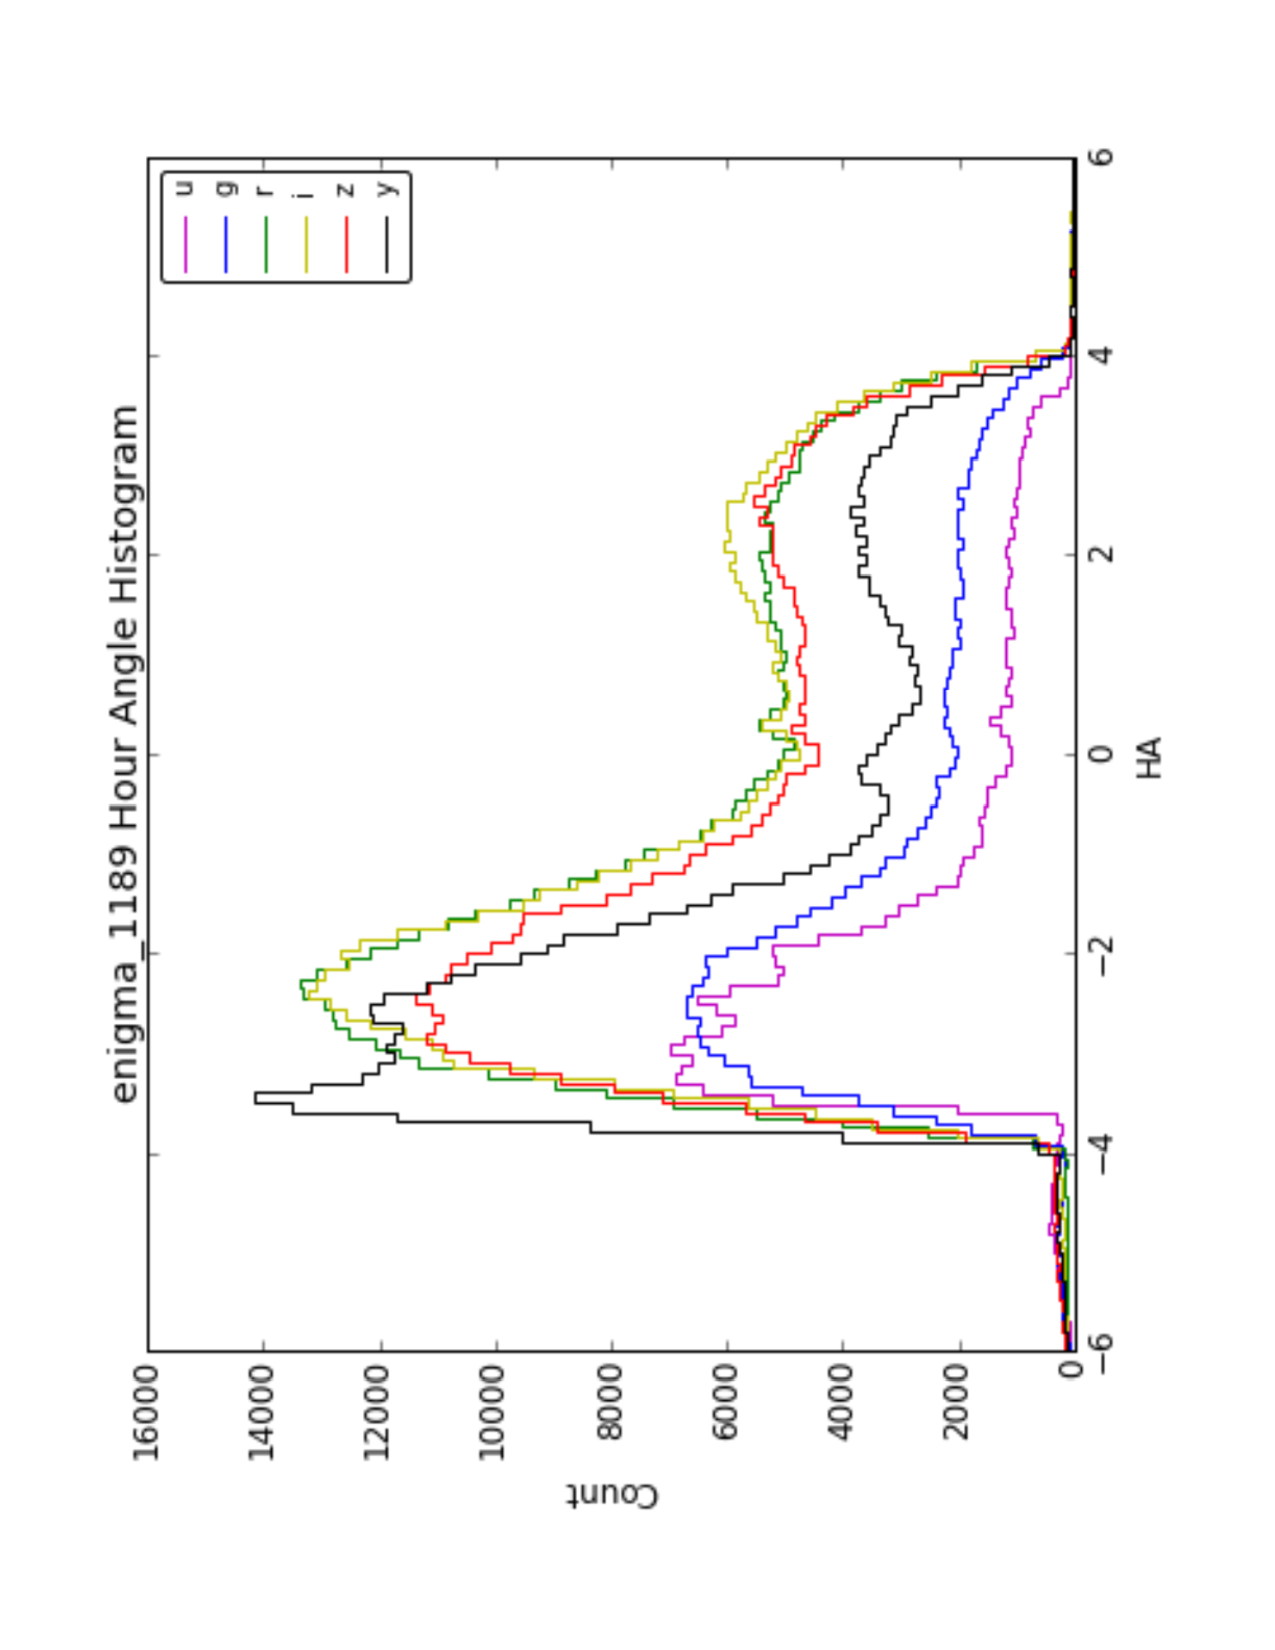
\includegraphics[angle=270,width=0.49\hsize:,clip]{figs/enigma1189_HA.pdf}
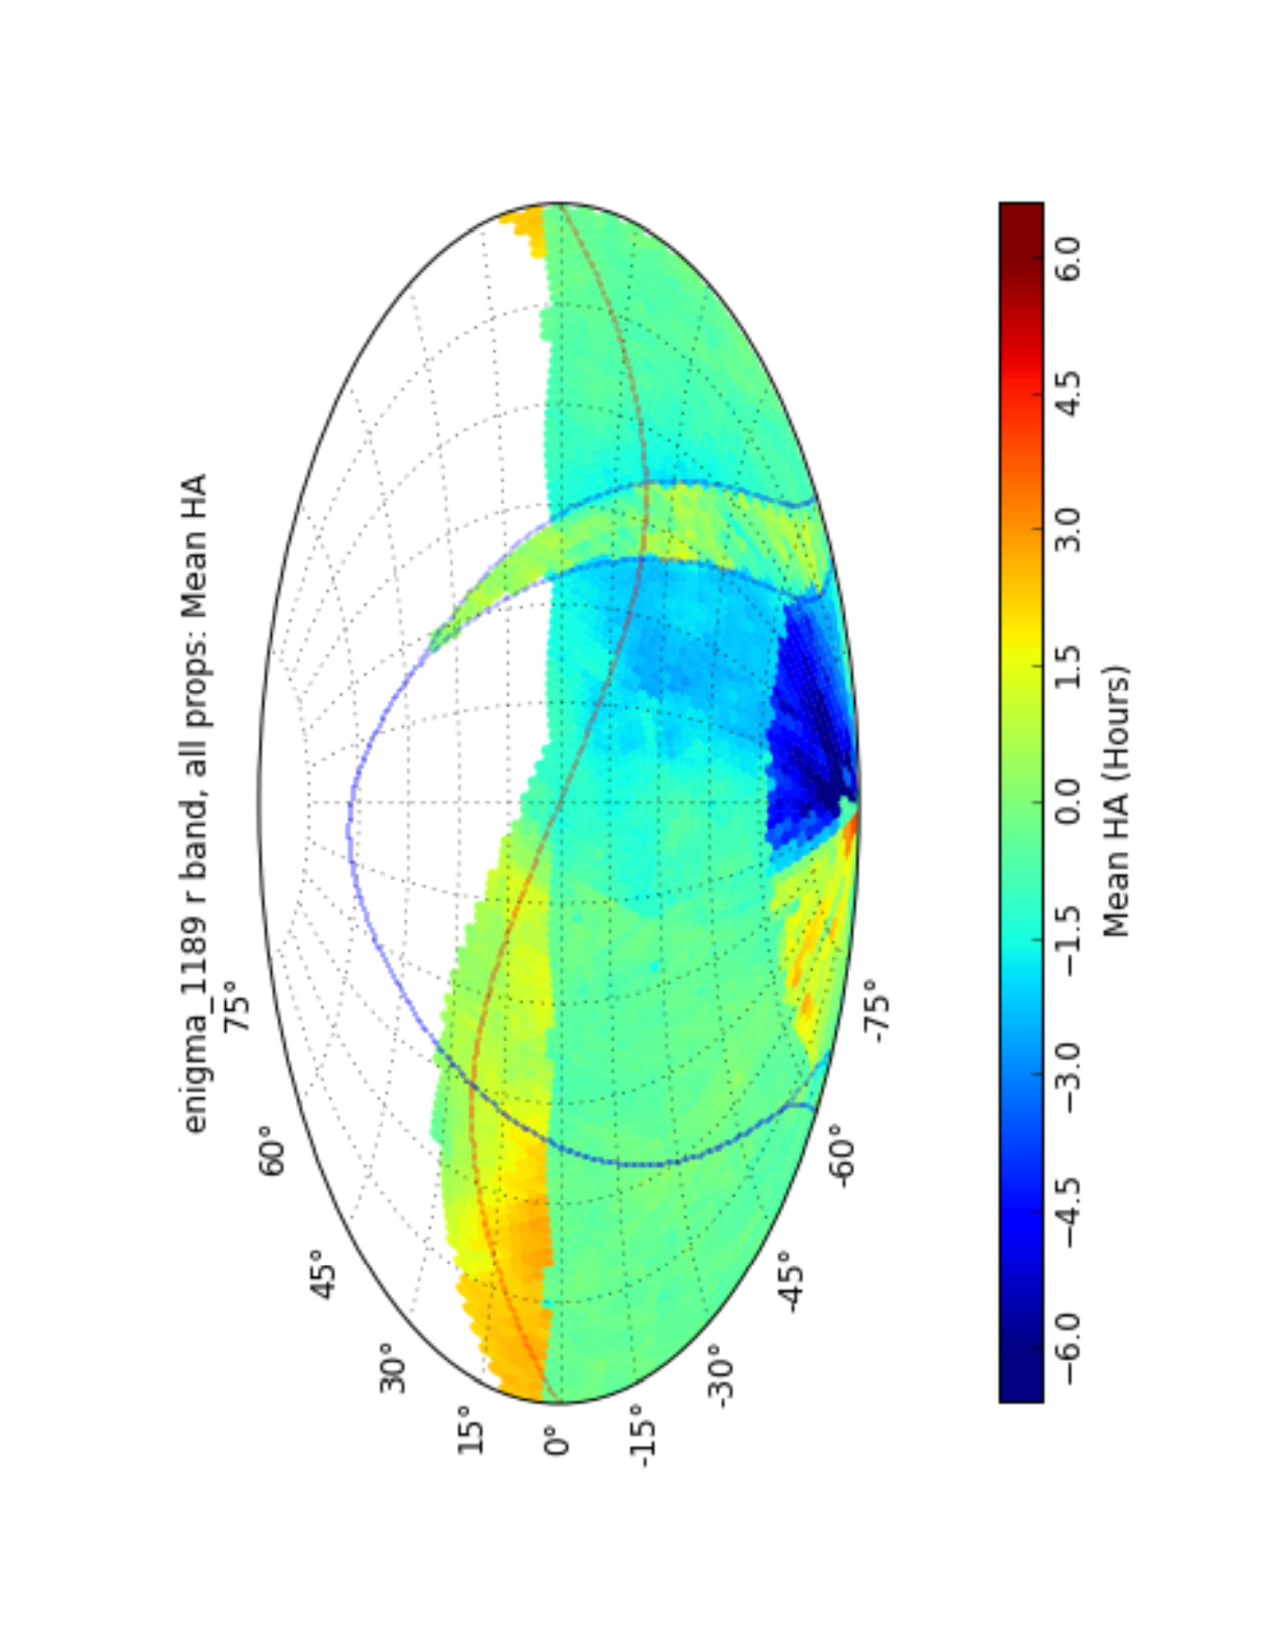
\includegraphics[angle=270,width=0.49\hsize:,clip]{figs/enigma1189_meanHA.pdf}
\vskip -0.3in
\caption{Histograms in the left panel show the distribution of hour angles (HA) in
6 bands for all proposals from simulated cadence \opsimdbref{db:enigma} (the distributions are
similar for WFD fields considered alone). Note the bias towards observations west from
the meridian. The right panel shows the distribution across the sky of the mean HA for
all observations in the $r$ band. }
\label{fig:HAenigma}
\end{figure}
%%%%%%%%%%%%%%%%%%%%%%%%%%%%%%%%%


The candidate replacement ``Baseline Cadence'' candidate,
\opsimdbref{db:enigma}, has the following basic
properties\footnote{See
http://tusken.astro.washington.edu:8080/summaryStats?runId=1}:
\begin{enumerate}
\item The total number of visits is 2,469,307, with 85.4\% spent on
the Universal proposal (the main deep-wide-fast survey), 6.4\% on the
North Ecliptic proposal, 1.7\% on the Galactic plane proposal, 2.1\%
on the South Celestial pole proposal, and 4.5\% on the Deep Drilling
cosmology proposal.
\item The median number of visits {\it per night} is 815, the range is
35 to 1104, with 3062 observing nights. The mean slew time is 6.9
seconds (median: 4.8 sec) and the total open shutter time is 4.06
Msec. The median total open shutter time (per night) as a fraction of
the observing time (the ratio of the open shutter time and the sum of
the open shutter time, readout time and slew time) is 73\%. The
25\%-75\% quartiles for the number of filter changes per night are 2
and 7, with the mean of 4.6. The total number of filter changes is
15,364.
\item In the $r$ band, the median seeing is 0.77 arcsec, the median
airmass is 1.23, and the median $5\sigma$ depth for point sources is
24.5. The variation of the median airmass for the $r$ band
observations with the position on the sky is shown in
\autoref{fig:airmassenigma}.
\item For the 2,293 fields (somewhat overlapping) from the Universal
Cadence area (also known as WFD -- wide, fast, deep), the median
number of visits in the $ugrizy$ bands is (63, 89, 202, 202, 182,
181), respectively. Not only that these medians exceed the requested
number of visits (design specification from the SRD\footnote{The LSST
Science Requirements Document (SRD) is available as
http://ls.st/lpm-17}) of (56, 80, 184, 184, 160, 160) in the $ugrizy$
bands, but the minimum number of visits per field over this area does
so, too. This result is quite encouraging given that only 85\% of
observing time was spent on the Universal Cadence proposal. The mean
number of visits over the Universal Cadence area, summed over all
bands, is 920.
\item The coadded $5\sigma$ depth\footnote{Note that these values
depend on externally supplied values for fiducial single-epoch
$5\sigma$ depths; the following values were used in analysis described
here: (24.45, 25.17, 24.67, 24.27, 23.57, 22.36) in the $ugrizy$
bands, respectively. These values are progressively deeper towards the
blue bands and shallower towards the red bands, compared to the values
listed in Table 2 from the latest version (v3.1) of the LSST overview
paper: (23.68 , 24.89, 24.43, 24.00, 23.45, 22.60). This discrepancy
is due to the Project software evolution falling behind continuing
improvements in the system performance estimates and will be rectified
by introducing automated version control system across the Project.}
for point sources in the $ugrizy$ bands is (26.1, 27.3, 27.4, 26.7,
25.4, 24.4), respectively. The distribution of coadded depth across
the sky is fairly uniform; for an example see
\autoref{fig:coaddm5enigma}.
\item For the 2,293 fields from the Universal Cadence area, the median
seeing is 0.75 arcsec in the $r$ band and 0.74 arcsec in the $i$ band.
The median airmass in the $urz$ bands is 1.25, 1.20 and 1.26 (the
maximum allowed airmass for the Universal Cadence area was set to
1.5).  The median sky brightness in the $ury$ bands is 22.0
mag/arcsec$^2$, 21.1 mag/arcsec$^2$, and 17.3 mag/arcsec$^2$,
respectively.
\item Restricted to the Universal Cadence fields, a unique area of
18,000 sq.deg. received at least 898 visits (summed over bands; the
SRD design value is 825).
\item The median trigonometric parallax and proper motion errors are
0.57 mas and 0.16 mas/yr, respectively, for bright sources (limited by
assumed systematic errors in relative astrometry of 10 mas), and 5.5
mas and 1.6 mas/yr for points sources with $r=24$ (assuming flat
spectral energy distribution), over the Universal Cadence fields. The
variation of parallax and proper motion errors across the sky is
visualized in \autoref{fig:parapmenigma}.
\end{enumerate}


%%%%%%%%%%%%%%%%%%%%%%%%%%%%%%%%%
\begin{figure}[t!]
\vskip -3.5in
\hskip -0.5in
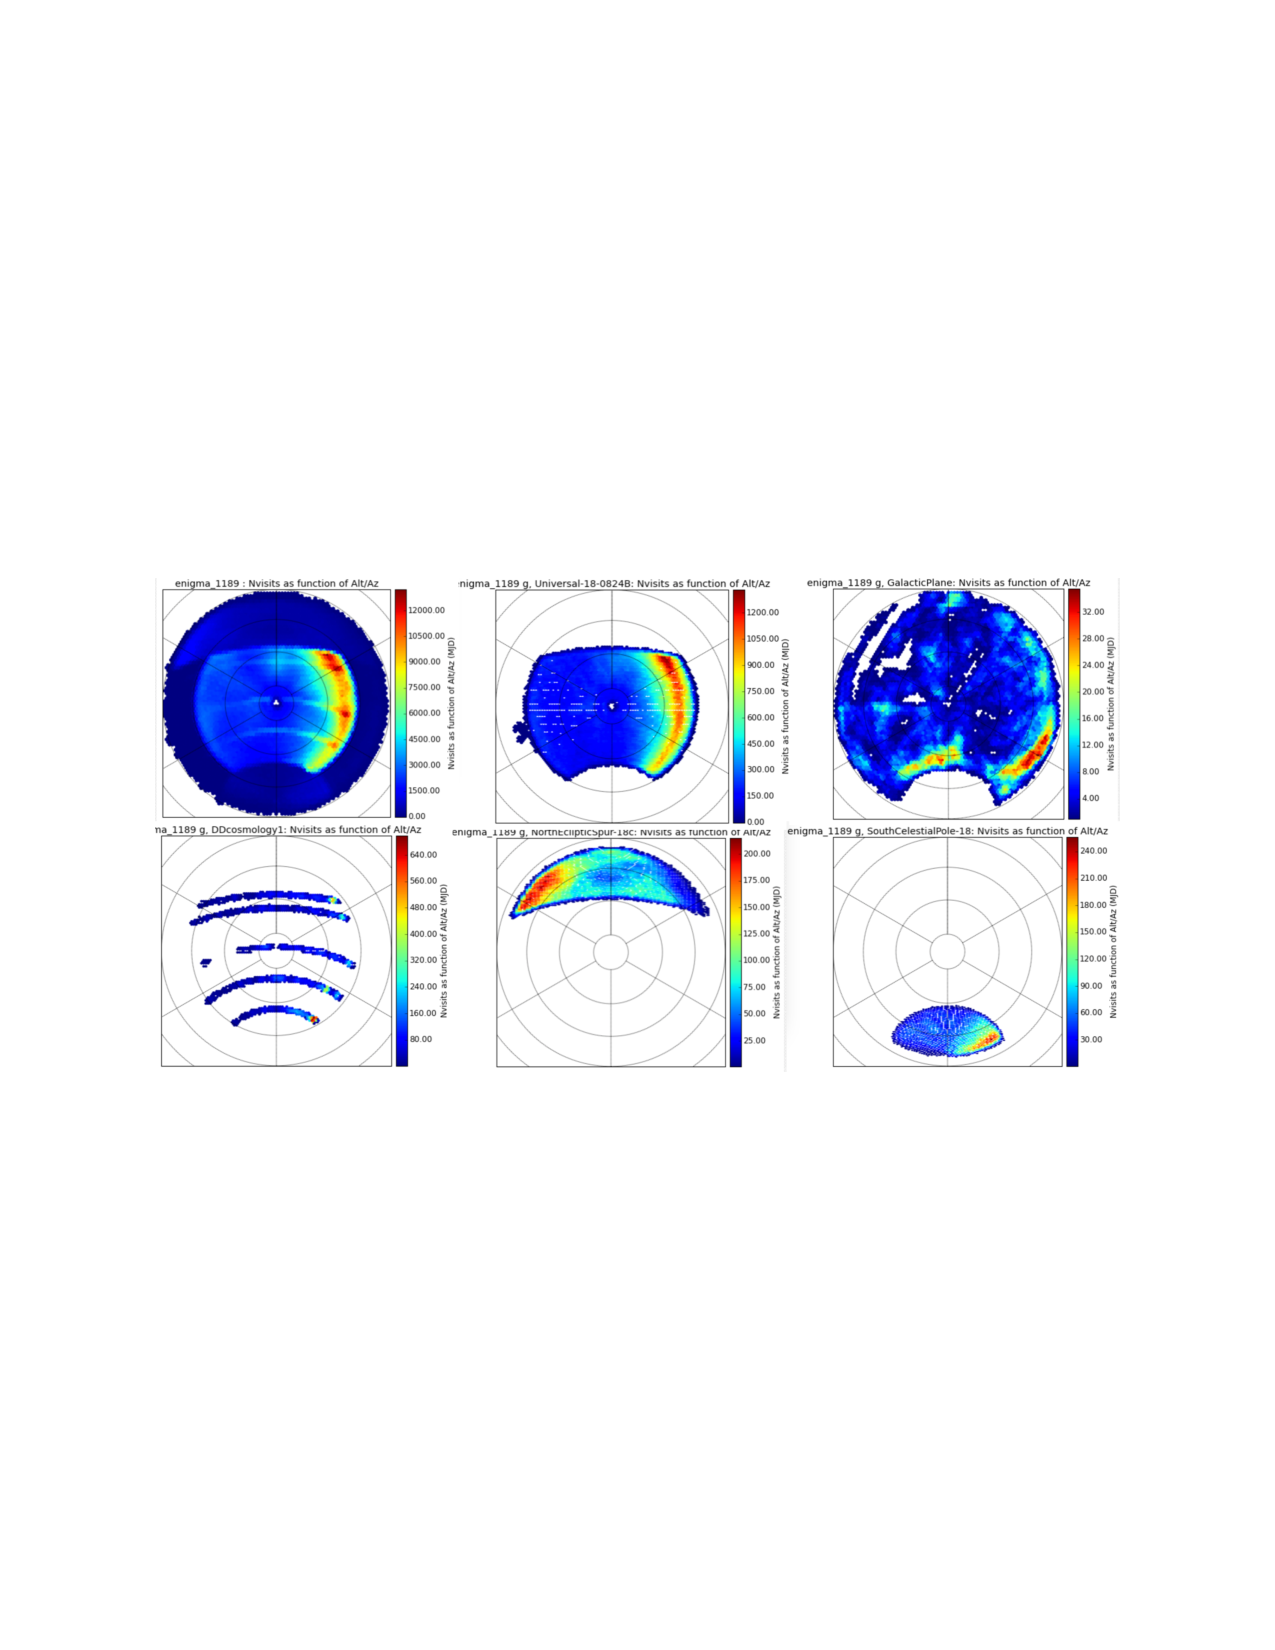
\includegraphics[angle=0,width=1.19\hsize:,clip]{figs/aaAllp.pdf}
\vskip -3.5in
\caption{The color-coded map in the top left panel shows the g band visit count from
Baseline Cadence simulation \opsimdbref{db:enigma} in the equal-area Lambert projection of the
horizontal coordinate system (altitude-azimuth), with north on top and west towards the
right. The horizon corresponds to the largest circle. Five implemented proposals are shown
separately in other panels (top row: Universal and Galactic Plane, bottom row: Deep Drilling
fields, North Ecliptic Spur, and South Celestial Pole region). The Universal cadence was
limited to airmass below 1.5, while other proposals sampled higher airmass, too (see the
histogram in \autoref{fig:airmassenigma}).  Note the strong propensity of Universal fields
for westward observations (the median airmass is about 1.2).}
\label{fig:AltAzenigma}
\end{figure}
%%%%%%%%%%%%%%%%%%%%%%%%%%%%%%%%%

%%%%%%%%%%%%%%%%%%%%%%%%%%%%%%%%%
\begin{figure}[b!]
\vskip -1.1in
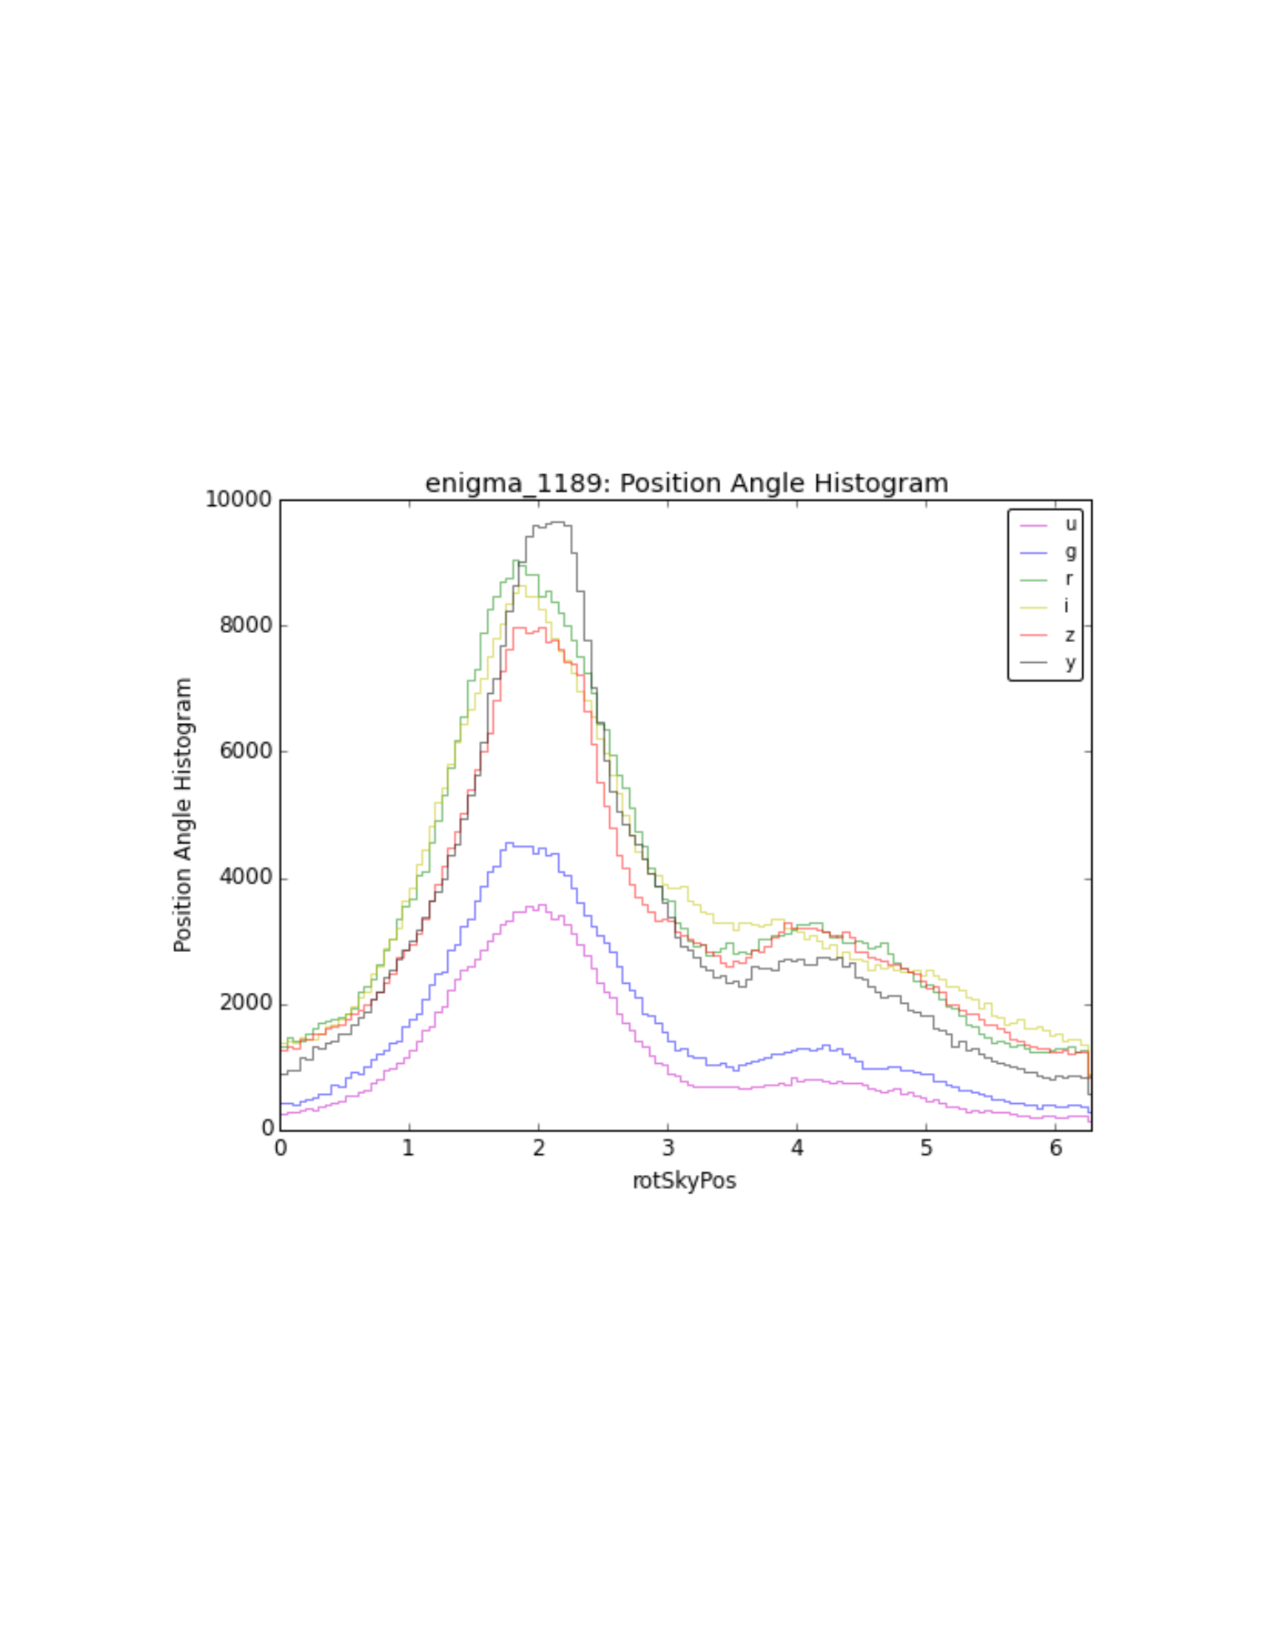
\includegraphics[angle=0,width=0.49\hsize:,clip]{figs/enigma1189_rotator.pdf}
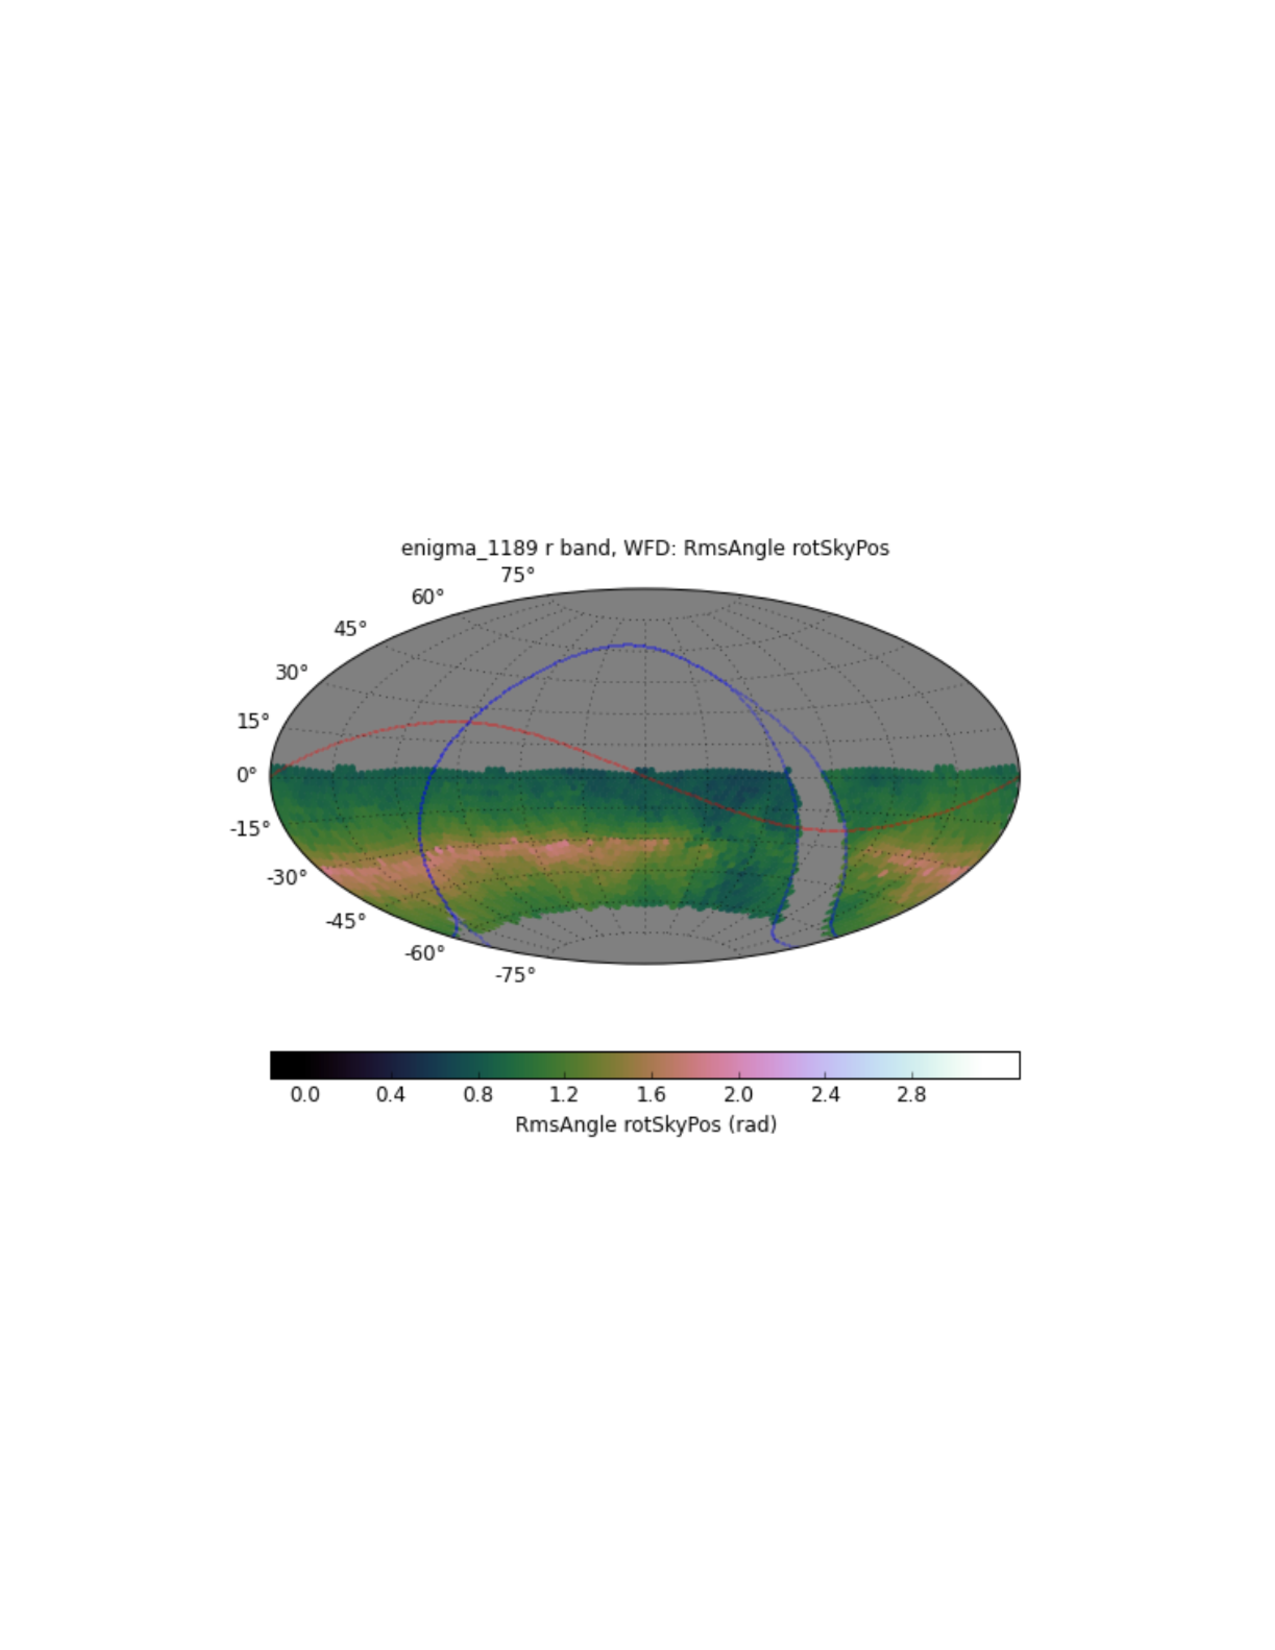
\includegraphics[angle=0,width=0.49\hsize:,clip]{figs/enigma1189_rotator2.pdf}
\vskip -1.3in
\caption{The left panel shows the position angle distribution (in radians)  in each band for the
main survey fields in \opsimdbref{db:enigma}. The position angle is the angle between ``up'' in the image
and North on the sky. The variation of the root-mean-square scatter of the $r$ band
distribution across the sky is shown in the right panel.}
\label{fig:rotator}
\end{figure}
%%%%%%%%%%%%%%%%%%%%%%%%%%%%%%%%%

%%%%%%%%%%%%%%%%%%%%%%%%%%%%%%%%%
\begin{figure}[t!]
\vskip -4.1in
\hskip -0.5in
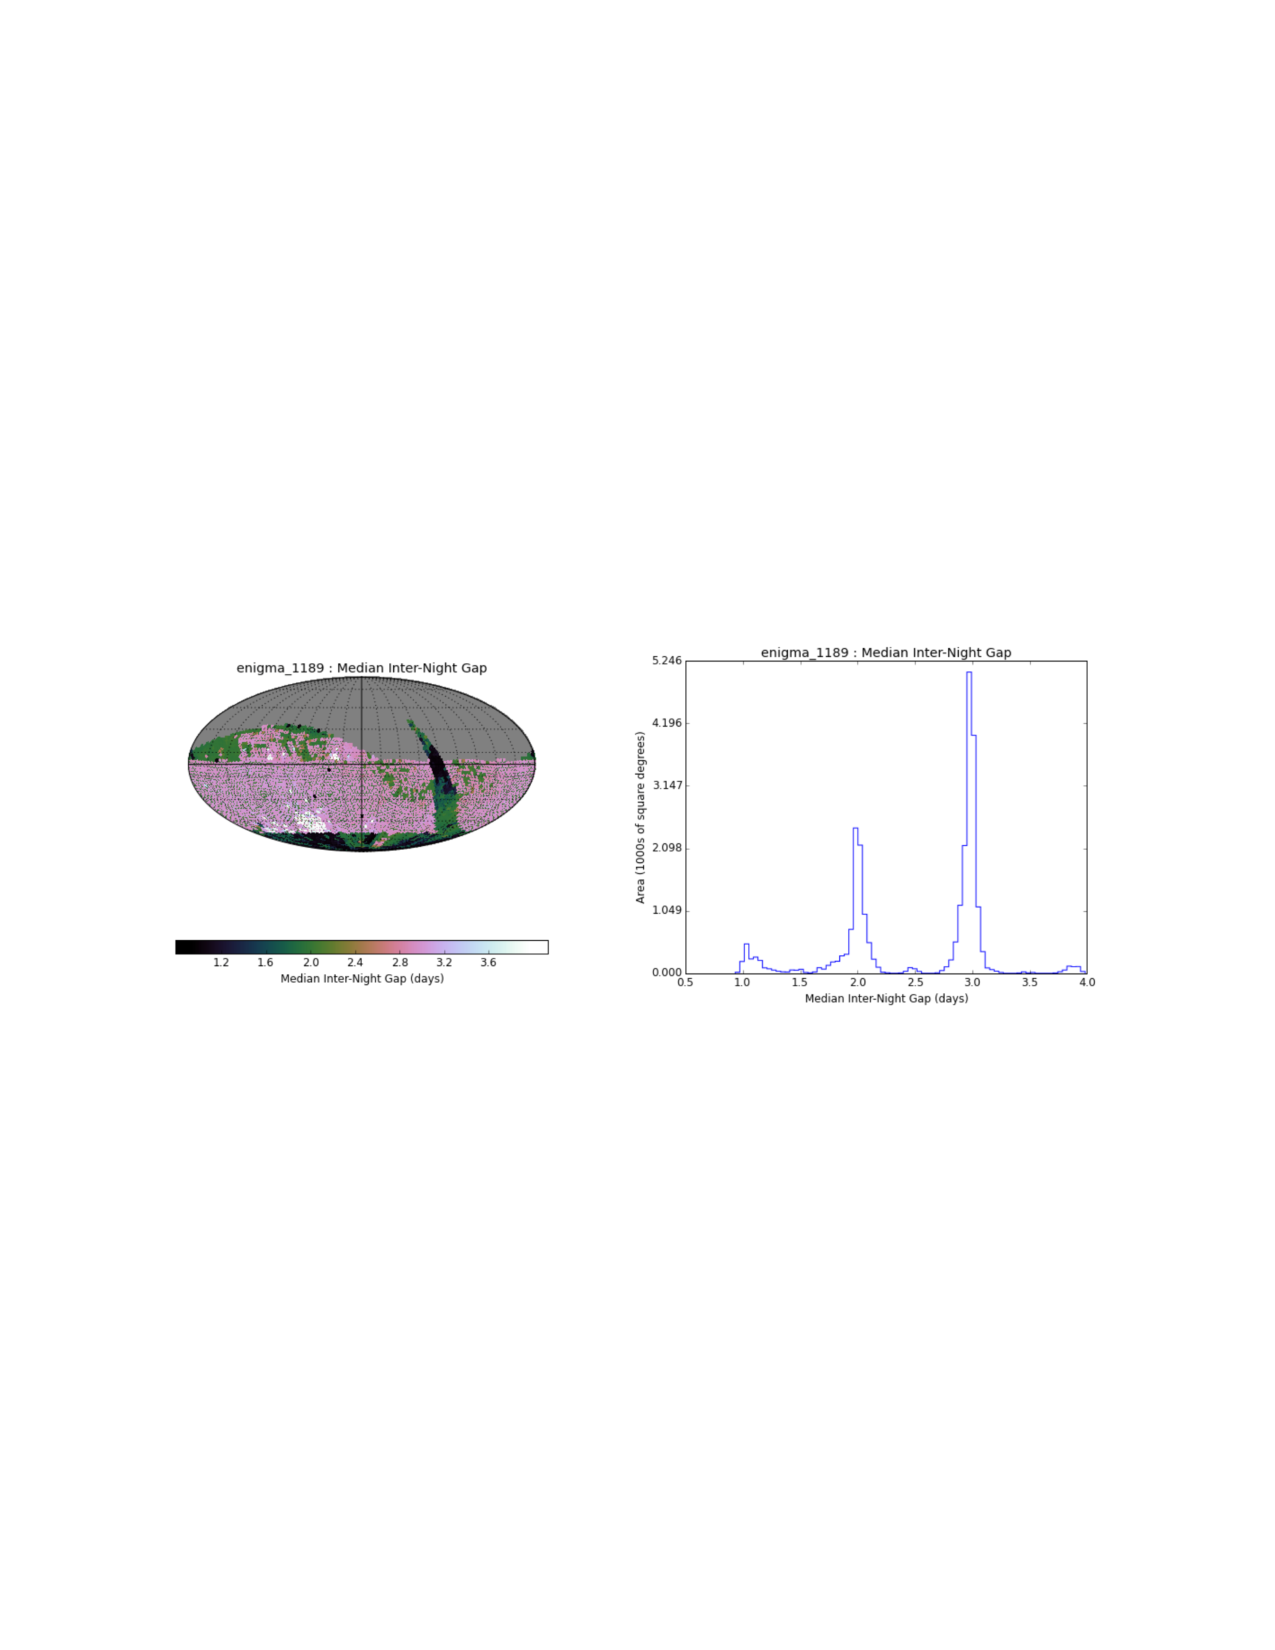
\includegraphics[angle=0,width=1.19\hsize:,clip]{figs/enigma1189_interGapAll.pdf}
\vskip -4.0in
\caption{The median inter-night gap (or revisit time) is shown in Aitoff projection
for all proposals and all filters for candidate Baseline Cadence \opsimdbref{db:enigma}.
On average, fields in the main survey get revisited about every 3 days.}
\label{fig:enigmaGapAll}
\end{figure}
%%%%%%%%%%%%%%%%%%%%%%%%%%%%%%%%%

%%%%%%%%%%%%%%%%%%%%%%%%%%%%%%%%%
\begin{figure}[h!]
\vskip -3.8in
\hskip -0.5in
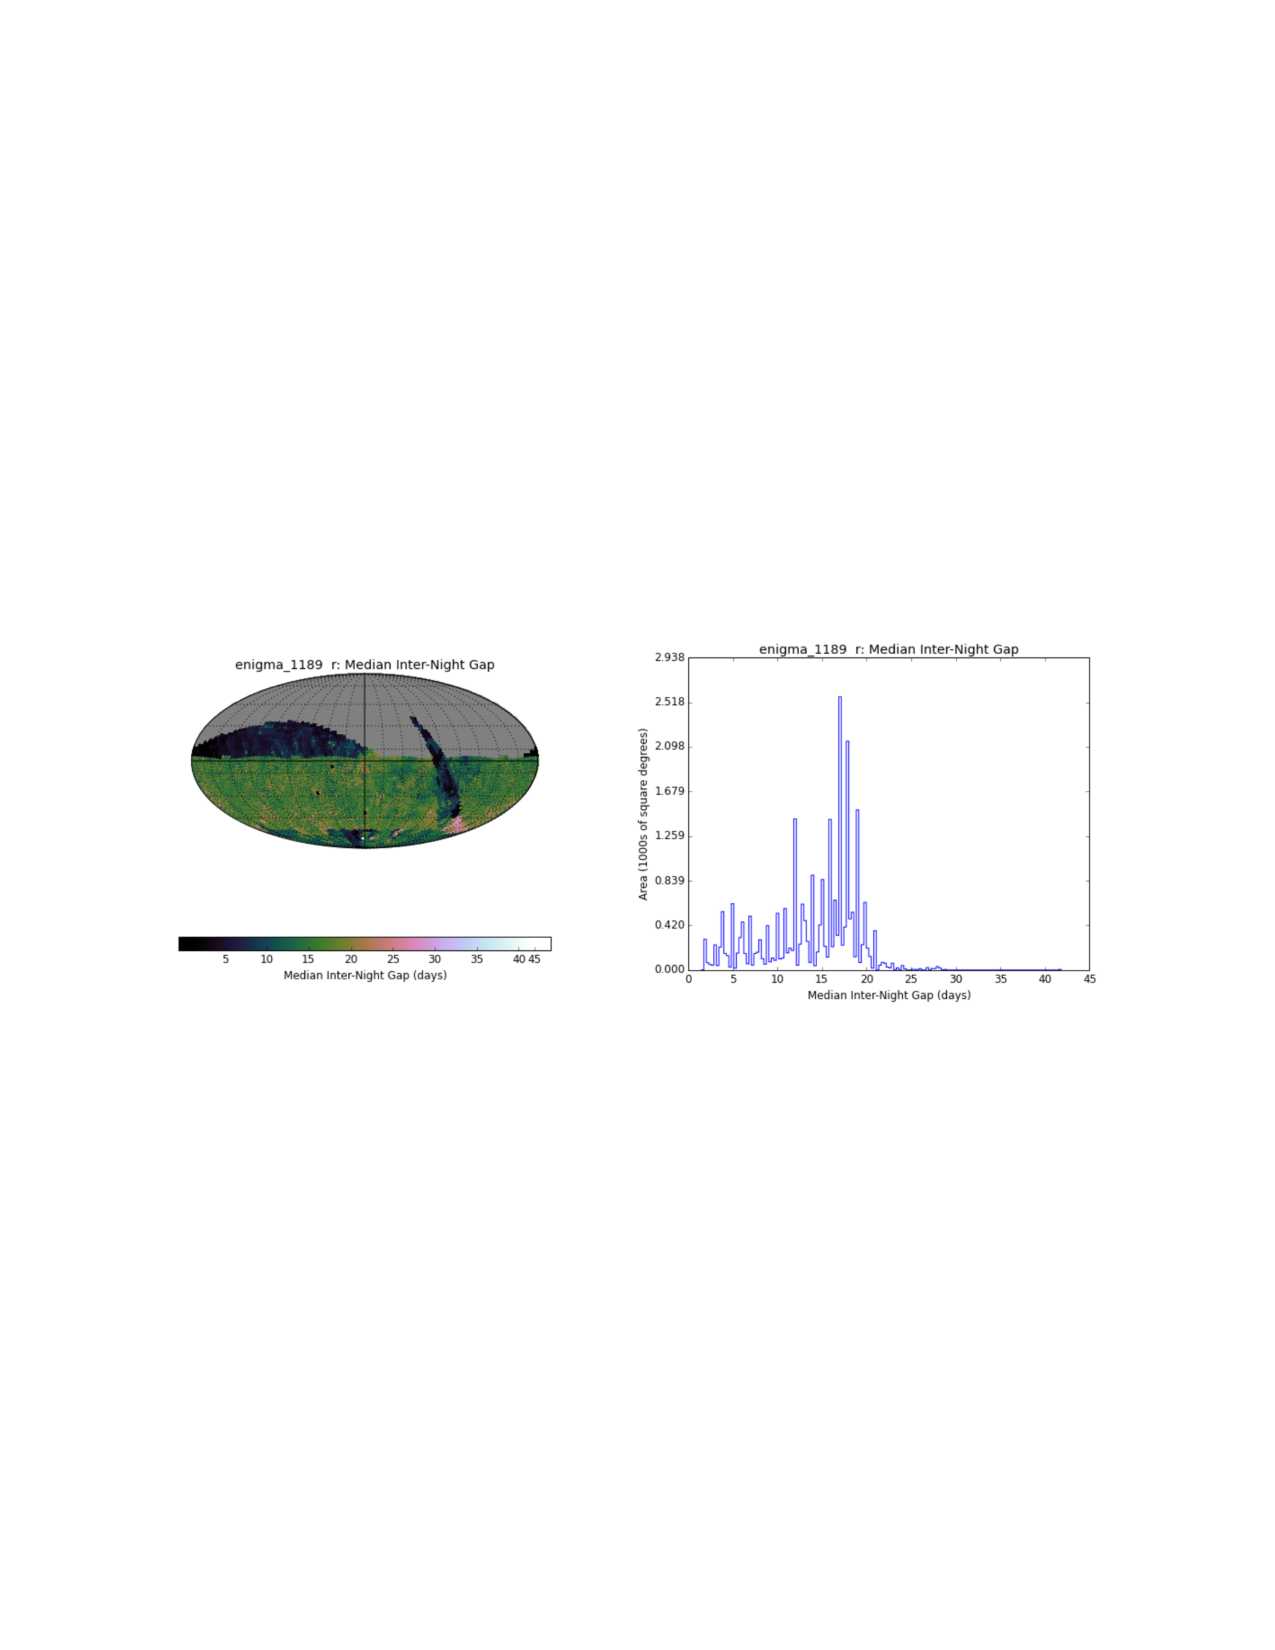
\includegraphics[angle=0,width=1.19\hsize:,clip]{figs/enigma1189_interGap_r.pdf}
\vskip -4.0in
\caption{The median inter-night gap for r band visits is shown in Aitoff projection
for all proposals and all filters for candidate Baseline Cadence \opsimdbref{db:enigma}.
On average, fields in the main survey get revisited in the r band about every 15 days.}
\label{fig:enigmaGapr}
\end{figure}
%%%%%%%%%%%%%%%%%%%%%%%%%%%%%%%%%

%%%%%%%%%%%%%%%%%%%%%%%%%%%%%%%%%
\begin{figure}[b!]
\vskip -3.8in
\hskip -0.5in
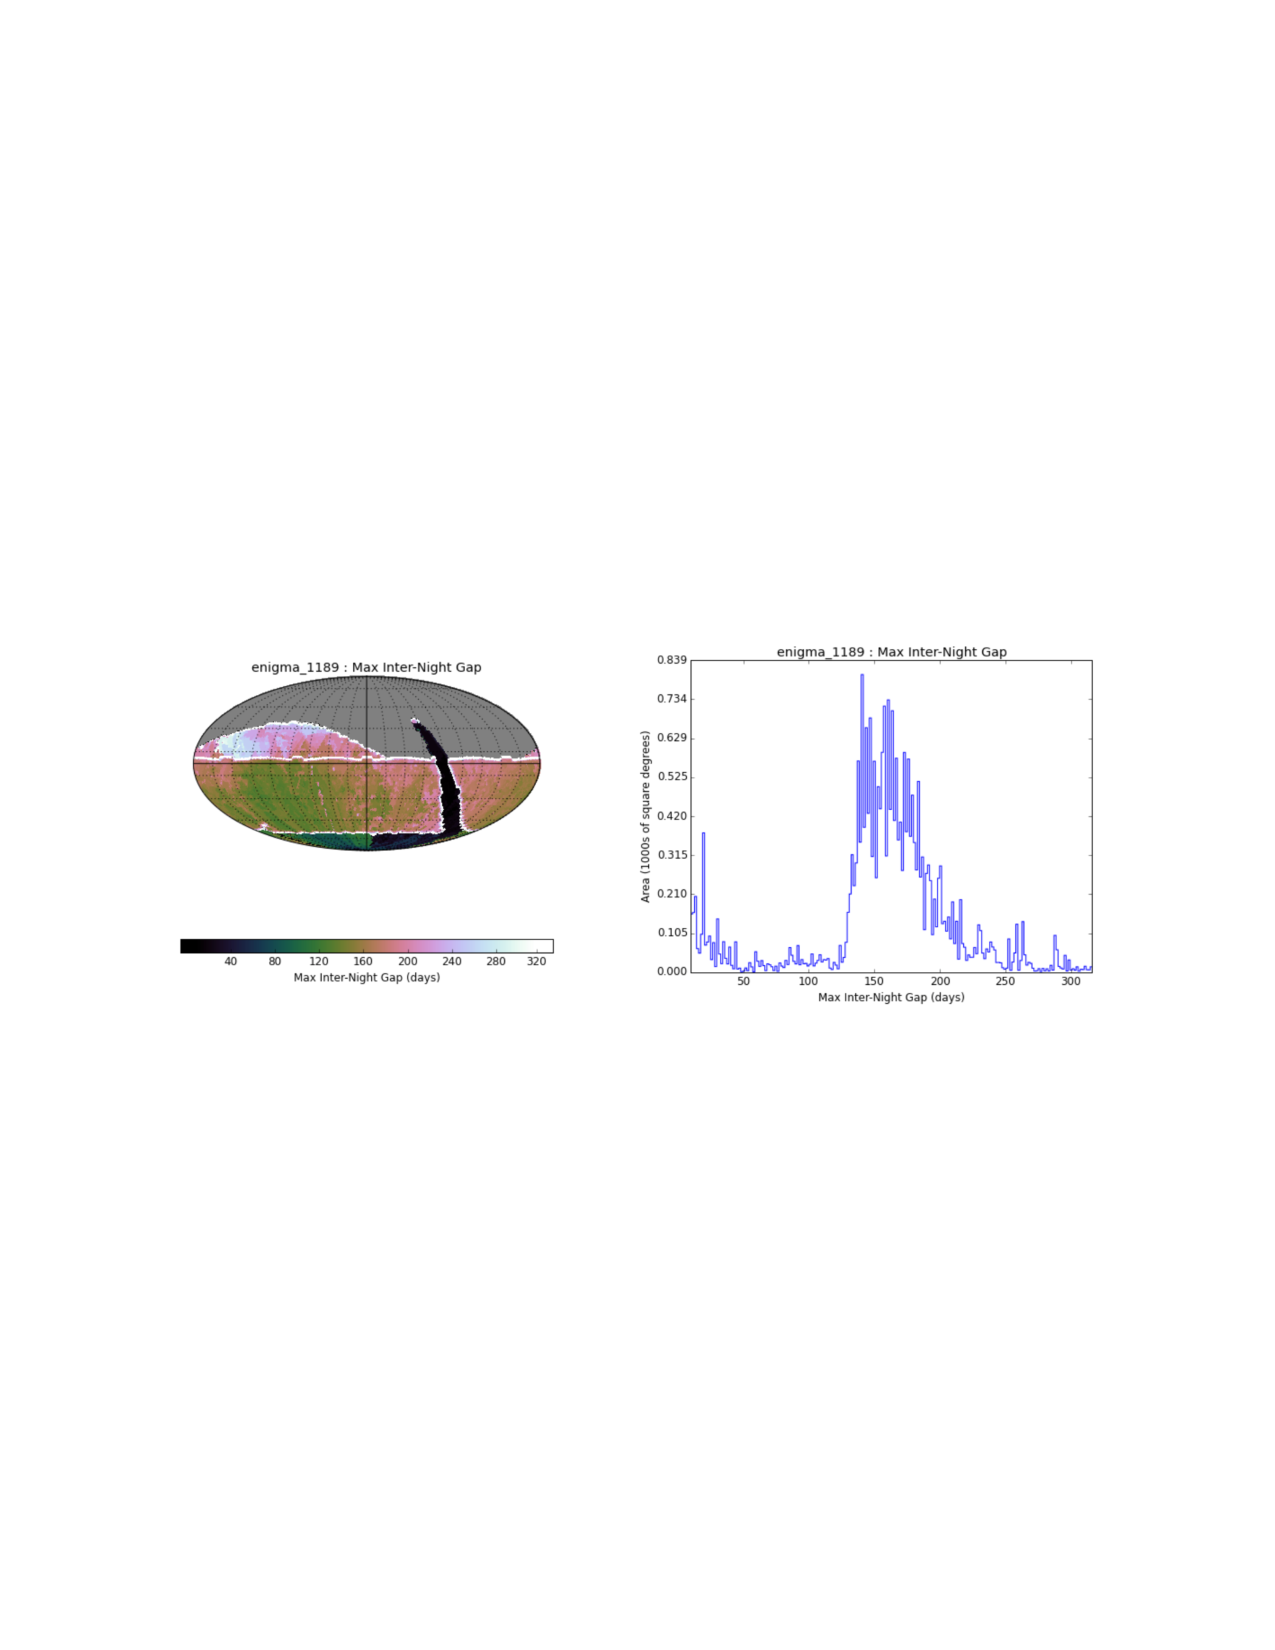
\includegraphics[angle=0,width=1.19\hsize:,clip]{figs/enigma1189_MAXinterGapAll.pdf}
\vskip -4.0in
\caption{The maximum inter-night gap (or revisit time) is shown in Aitoff projection
for all proposals and all filters for candidate Baseline Cadence \opsimdbref{db:enigma}.}
\label{fig:enigmaMAXGapAll}
\end{figure}
%%%%%%%%%%%%%%%%%%%%%%%%%%%%%%%%%

%%%%%%%%%%%%%%%%%%%%%%%%%%%%%%%%%
\begin{figure}[t!]
\vskip -4.1in
\hskip -0.5in
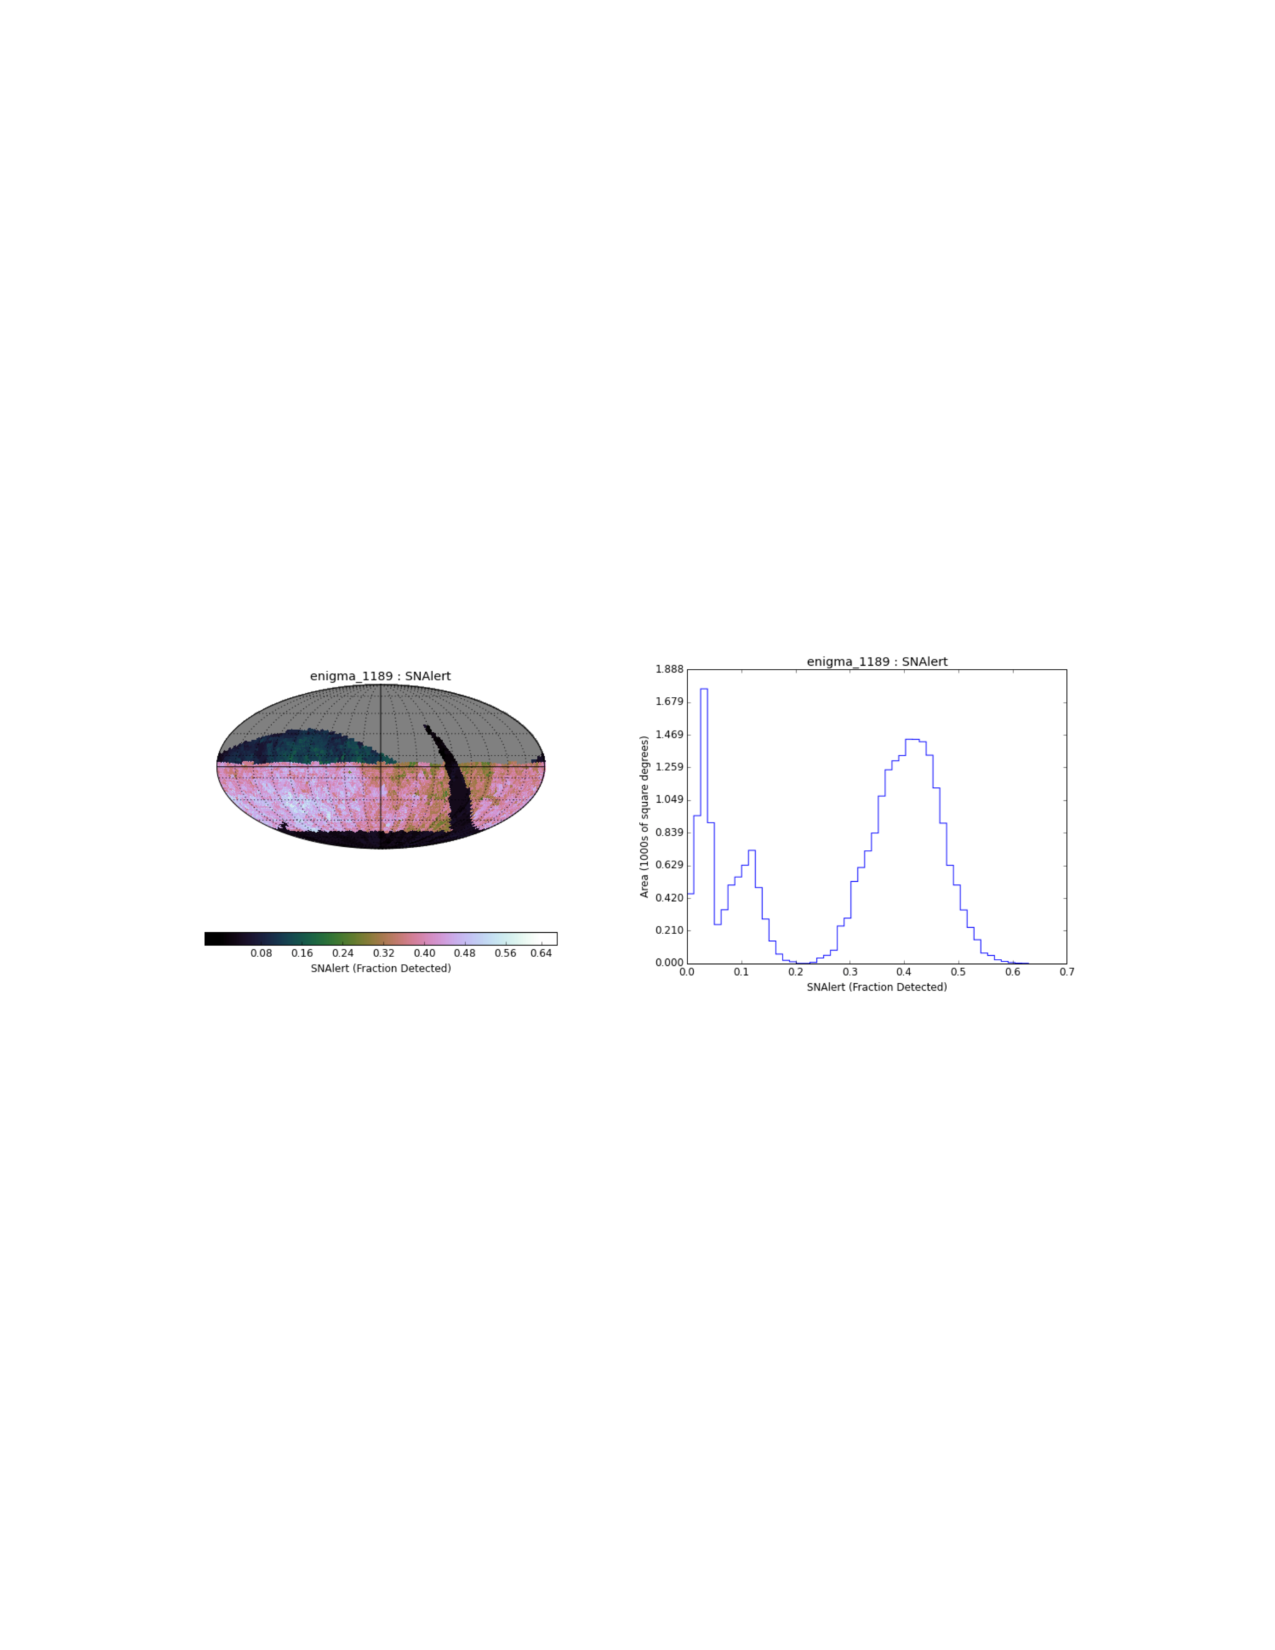
\includegraphics[angle=0,width=1.19\hsize:,clip]{figs/enigma1189_earlySNe.pdf}
\vskip -4.0in
\caption{The fraction of simulated Type Ia SNe at a redshift of 0.5 detected
pre-peak in any filter for candidate Baseline Cadence \opsimdbref{db:enigma}. About
40\% of all such SNe from the main survey will be detected before their
maximum brightness.}
\label{fig:enigmaEarlySNe}
\end{figure}
%%%%%%%%%%%%%%%%%%%%%%%%%%%%%%%%%


For comparison, the current Baseline Cadence, \texttt{opsim3.61}
(obtained with old OpSim code), delivered 2,651,588 visits, or 7.4\%
more than \opsimdbref{db:enigma}  (this is due to known effects and
changes in the code,  such as more pre-scheduled down time in the new
version). Perhaps the most important (and undesired!) difference
between the two simulations is that the new candidate Baseline Cadence
spent 6.4\% of the observing time on North Ecliptic Spur proposal (vs.
4\% spent on corresponding Universal North proposal in
\texttt{opsim3.61}), and less than 90\% of time on the Universal
proposal (the main wide-deep-fast survey).

Analysis of the hour angle distribution, shown in
\autoref{fig:HAenigma} and \autoref{fig:AltAzenigma}, reveals a strong
bias towards observations west from the meridian for the main survey.
{\it This pattern is not fully understood at this time} and may be
caused by specific features of the cost function implemented in the
OpSim code.

Another potentially undesireable feature, seen in practically all
simulations analyzed here, is that up to about a quarter of visits in
the main survey area represents the third, the fourth and sometimes
even the fifth visit to a field in the same night. For a large number
of time-domain programs, these visits could be used instead to
decrease the field inter-night revisit time. For more details, see
\autoref{sec:cadexp:NEOs}. The position angle distributions for this simulation
are shown in \autoref{fig:rotator}.


\subsubsection{Time-domain metrics}

The analysis of metrics designed for time-domain science has not been
performed yet in detail, except for the analysis of asteroid
completeness discussed in \autoref{sec:cadexp:NEOs}. MAF already includes
several sophisticated metrics, e.g., period recovery for variable
stars, which will be described in a later version of this report.

As a brief illustration of time-domain analysis,
\autoref{fig:enigmaGapAll} shows the median revisit time distribution
when all bands are considered, and \autoref{fig:enigmaGapr} shows the
median revisit time distribution in the band.  On average, fields in
the main survey get revisited about every 3 days using all filters,
and every 15 days when using only r band visits (30 days when using
only u band visits is the longest median revisit time).
\autoref{fig:enigmaMAXGapAll} shows the maximum inter-night gap, which
on average is about 5-6 months.

The temporal sampling for this simulation is sufficient to enable a
large recovery fraction for SNe. \autoref{fig:enigmaEarlySNe} shows
that a large fraction of LSST SNe will be detected before their
maximum brightness. Similar MAF metrics that explore various quality
cuts on SNe light curves (e.g. ``detected at least 6 times, at least 3
pre-peak, at least 3 post-peak, with observations in at least 3
filters'').

Intra-night revisit time distribution is discussed in more detail in
\S\ref{sec:cadexp:NEOs}.


\subsubsection{Special Proposals}

Regarding the special proposals, here we only provide the basic
performance parameters. With the exception of the Deep Drilling
proposal, these proposals are essentially strawman placeholders. The
North Ecliptic proposal (6.4\% of the observing time) obtained an
additional 300 visits per field, summed over $griz$ bands. These
fields are placed along the northern part of the Ecliptic. The
Galactic plane proposal (1.7\%) obtained 30 visits per band in all six
bands, across the region extending in Galactic latitude 10 degrees
from the Galactic center, with the boundary approaching the Galactic
equator linearly with longitude, and the zone ending at $l=90$ deg.
and at $l=270$ deg. The South Celestial pole proposal (2.1\%) obtained
30 visits per band in all six bands, for fields centers with Dec $<
-62.5$ deg. The Deep Drilling cosmology proposal (4.5\%) included 5
fields, with each obtaining several thousand visits per band. The
coadded $5\sigma$ depths for these fields are much fainter than for
the main survey: the medians values are (28.5, 28.6, 28.8, 28.2, 27.7,
26.0) in the $ugrizy$ bands, respectively.


\vskip 0.2in
{\bf Conclusions:}

The candidate “Baseline Cadence”, \opsimdbref{db:enigma}, appears to
be an adequate replacement for the current baseline cadence
(\texttt{opsim3.61}). Based on this preliminary analysis, there are no
major problems with its performance. While there are patterns which
are not fully understood (most notably the observing bias towards
west),  or undesired (unnecessary revisits of the same field in the
same night), \opsimdbref{db:enigma} is used as a benchmark cadence,
and referred to as ``Baseline Cadence'',  in the rest of this
document\footnote{Assuming that additional analysis will not uncover
any major deficiencies, this simulation will be discussed by the
Project Science Team and proposed for adoption as the new Baseline
Cadence to the Change Control Board. The target date for this proposal
is late September 2015.}

An important feature of \opsimdbref{db:enigma} simulation is that the
mean slew time of 6.9 sec is very close to the minimum possible slew
time of about 4.5 sec. The implication is that the surveying
efficiency, assuming 30 sec exposure time per visit, can be increased
by at most about 6\% (that is, the total open-shutter time is within
about 6\% from its possible maximum, given everything else unchanged).
Nevertheless, there are other survey aspects, including sky coverage
and temporal sampling functions, that can be further optimized, as
discussed in \autoref{sec:CE}.

\navigationbar

% --------------------------------------------------------------------

\section{Some Simulated Alternative Observing Strategies}
\def\secname{cadexp:alternatives}\label{sec:\secname}

We now describe some alternatives to the Baseline Cadence that were
explored. These \OpSim databases are all available for further testing
with science-based MAF metrics.

% - - - - - - - - - - - - - - - - - - - - - - - - - - - - - - - - - -

%%%%%%%%%%%%%%%%%%%%%%%%%%%%%%%
\opsimdb[db:opstwo]{ops2\_1098}{Only Universal Cadence, with pairs of visits.}
%%%%%%%%%%%%%%%%%%%%%%%%%%%%%%%

{\bf Motivation and description:} Formally, $\sim$90\% of observing
time is allocated to the main Universal Cadence program (WFD). The
remaining observing time is allocated to other programs, such as
``Deep Drilling'' programs (see Section 3.4 and Tables 22-26  in the
SRD). With this simulation, we wished to find out what would be the
effect of ignoring special programs and spending all of the observing
time on the main Universal Cadence program. \\

{\bf Expectations:} About 2.11 million visits (85\% of 2.47 million
visits) from Baseline Cadence (\opsimdbref{db:enigma}) were allocated
to WFD cadence. Here we expect that all of these 2.47 million visits
will be allocated to WFD cadence. \\

{\bf Analysis Results:} This simulated cadence is named \opsimdbref{db:opstwo}.
Compared to the Baseline Cadence \opsimdbref{db:enigma}:
\begin{enumerate}
\item The total number of visits is close to the expected value: 2.45 million.
The minimum number of visits per field for the 2,293 WFD fields in Baseline Cadence
is 968 for this simulation, compared to 898 for Baseline Cadence.
\item The median number of visits per night and the mean slew time are
essentially the same as for Baseline Cadence (810 vs. 815 and 7.2 sec vs. 6.9 sec).
\item The median seeing, sky brightness and airmass in the r and i bands are
      essentially the same as for WFD fields in Baseline Cadence.
\item The median trigonometric parallax and proper motion errors are improved by
about 8\%, with improvements commensurate with the increase in the number of visits.
\item This simulation also shows observing bias towards west (that is, additional
special programs in \opsimdbref{db:enigma} are not reponsible for this bias).
\end{enumerate}


{\bf Conclusions:} \opsimdbref{db:opstwo}, using only uniform cadence
proposal, delivered 99.2\% of the number of visits obtained by
Baseline Cadence. Therefore, {\it the ``filler'' aspect of other
proposals does not have a major impact on the surveying efficiency}.
The minimum number of visits per field for the 2,293 WFD fields in
Baseline Cadence is 968 (the SRD design value is 825 and the stretch
goal value is 1000). Although the sky coverage of these 2293 fields is
about 18,000 sq.deg., their cumulative area is 22,000 sq.deg. With
proper dithering, the effective number of visits could be increased to
968*22/18 = 1183 (or the WFD area increased from 18,000 sq. deg.; see
analysis of ops2\_1092 below). This increase is an improvement of 43\%
relative to the SRD design specification of 825 visits over 18,000
sq.deg. However, note again that there are no other programs in this
simulation (i.e., if other programs were allocated 10\% of the
observing time, the implied overall ``over-performance'' in the number
of  visits would be about 30\%).

% - - - - - - - - - - - - - - - - - - - - - - - - - - - - - - - - - -

%%%%%%%%%%%%%%%%%%%%%%%%%%%%%%%%%
\opsimdb[opstwoPS]{ops2\_1092}{A Pan-STARRS-like observing strategy.}
%%%%%%%%%%%%%%%%%%%%%%%%%%%%%%%%%

{\bf Motivation and description:} "Pan-STARRS-like cadence” attempts
to apply a uniform cadence strategy throughout the survey region,
which is maximized and defined by Dec $< +15$ deg (about 27,400
deg$^2$). The maximum acceptable airmass is kept at its default value
of 1.5 (which excludes fields with Dec $< -78$ deg and Dec $> +18$
deg. This simulation utilizes uniform cadence and no other proposal,
and requires pairs of visits as in Baseline Cadence. \\

{\bf Expectations:} The total number of visits should be roughly the
same as in Baseline Cadence, but spread over a 42\% larger sky area
(3,255 fields instead of 2,293), with fewer visits per field. \\

{\bf Analysis Results:}  This simulated cadence is named \opsimdbref{db:opstwoPS}.
Compared to the Baseline Cadence \opsimdbref{db:enigma}:
\begin{enumerate}
\item The total number of visits is 2.47 million, and essentially identical to the
number of visits in Baseline cadence.
\item
The mean number of visits per field is 758.5, which is 98\% of the number of visits
for WFD fields obtained by Baseline Cadence (but here the sky area is 42\% larger).
\item The median number of visits per night and the mean slew time are
essentially the same as for Baseline Cadence.
\item The median seeing, sky brightnes and airmass in the r and i bands for WFD fields are
         essentially the same as in Baseline Cadence.
\item The median trigonometric parallax and proper motion errors show
uniform behavior over the entire enlarged area (see \autoref{fig:parapmenigma2}),
with the values similar to those obtained for Baseline Cadence.
\item This simulation also shows observing bias towards west.
\end{enumerate}

Due to increased sky area, which samples regions that can never
achieve low airmass, the median coadded depth is about 0.15 mag
shallower for this simulation than for Baseline Cadence. As a result,
the counts of galaxies per unit area down to a fixed SNR would
decrease by about 15-20\%. At the same time, the area outside the
Galactic plane is increased by about 30\%, and thus the total number
of galaxies would be increased by about 10\%, compared to WFD fields
in Baseline Cadence. However, the increased median airmass also
results in larger seeing, especially for the borderline regions, as
illustrated in \autoref{fig:PS-seeing}. The increased median seeing
would decrease the number of galaxies effectively resolved for weak
lensing by about 3-5\%. In addition, the additional area has somewhat
larger extinction due to interstellar dust which further decreases the
galaxy counts (this impact of dust extinction is not yet implemented
in MAF). As a result of these effects, the two strategies result in
similar weak lensing galaxy samples.

{\bf Conclusions:} When only the Universal Cadence proposal is
employed, the survey area could be increased by about 40\%, while
still delivering the mean number of fields at the level of 98\% of
that in Baseline Cadence (or 92\% of the SRD design value of 825).
Hence, simulations ops2\_1092  and \opsimdbref{db:opstwo} demonstrate
that the ``survey reserve'', relative to the Universal Cadence design
specifications from the SRD, can be used to i) increase the number of
visits per field over the WFD area,  or ii) increase the surveyed area
while keeping the number of visits per field statistically unchanged,
or iii) increase both area and the number of visits, and/or iv)
execute additional programs (the current baseline).


%%%%%%%%%%%%%%%%%%%%%%%%%%%%%%%%%
\begin{figure}[t!]
\vskip -0.03in
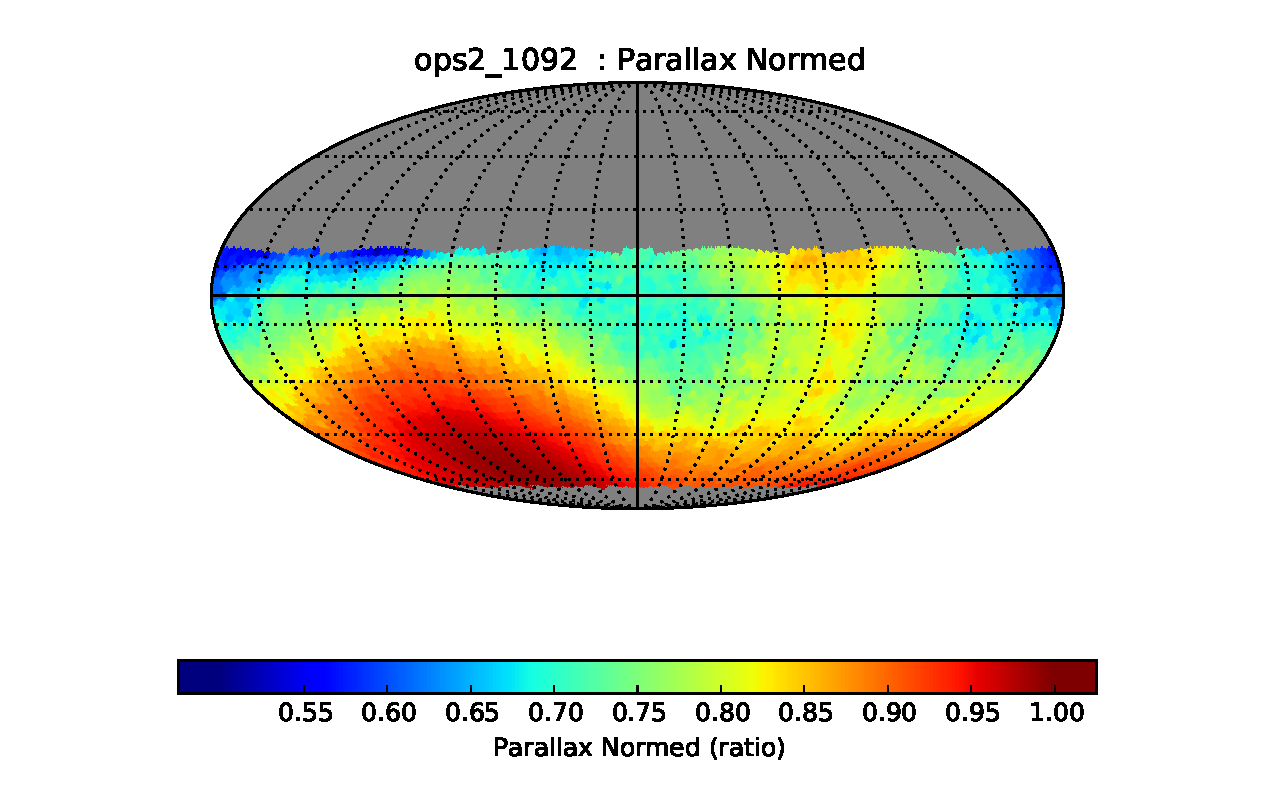
\includegraphics[angle=0,width=0.49\hsize:,clip]{figs/ops2_1092_Parallax_Normed__HEAL_SkyMap.pdf}
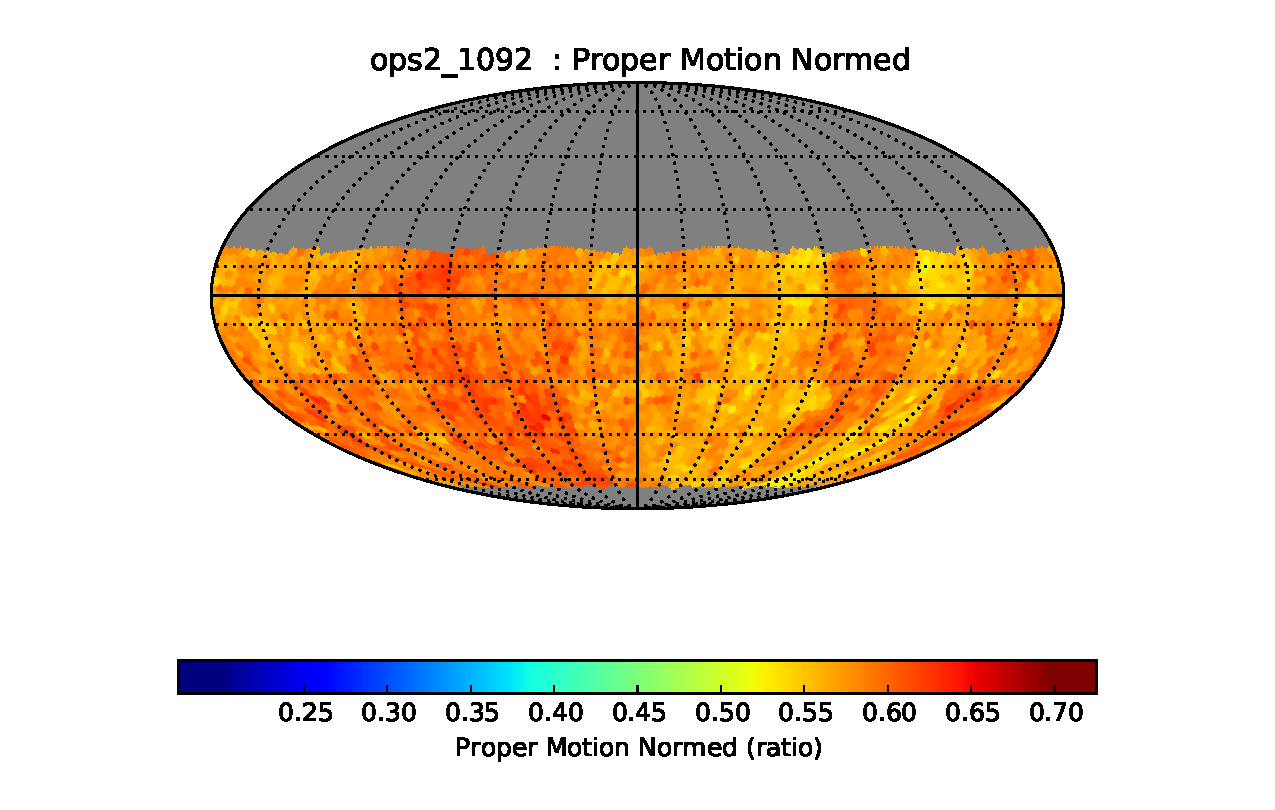
\includegraphics[angle=0,width=0.49\hsize:,clip]{figs/ops2_1092_Proper_Motion_Normed__HEAL_SkyMap.pdf}
\vskip -0.2in
\caption{The trigonometric parallax errors (left) and proper motion errors (right)  for simulated cadence
ops2\_1092 (``Pan-STARRS-like'' cadence), normalized by the values for idealized perfectly optimized
cadence, are shown in Aitoff projection of equatorial coordinates (compare to \autoref{fig:parapmenigma}).}
\label{fig:parapmenigma2}
\end{figure}
%%%%%%%%%%%%%%%%%%%%%%%%%%%%%%%%%

%%%%%%%%%%%%%%%%%%%%%%%%%%%%%%%%%
\begin{figure}[t!]
\vskip -3.9in
\hskip -0.5in
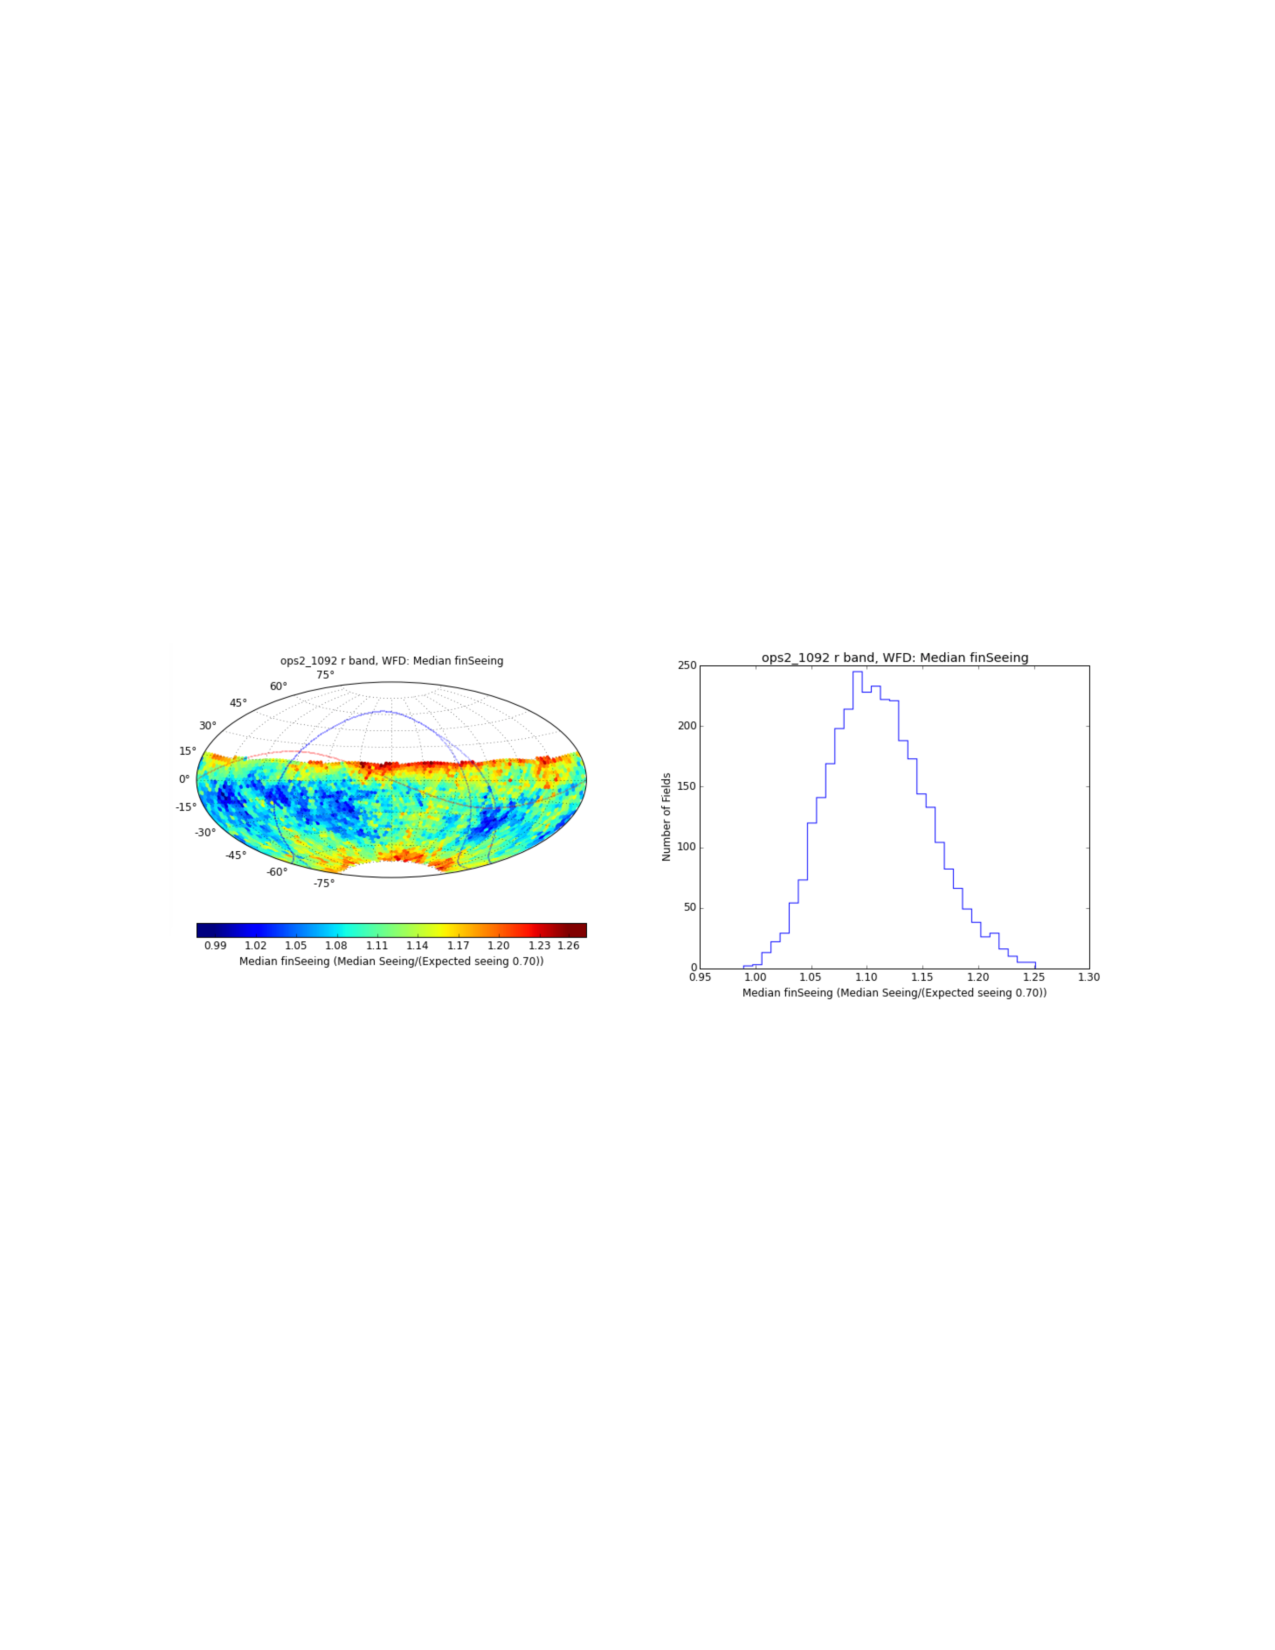
\includegraphics[angle=0,width=1.19\hsize:,clip]{figs/PS-seeing.pdf}
\vskip -4.0in
\caption{The median seeing in r filter, for simulated cadence ops2\_1092 (``Pan-STARRS-like'' cadence),
normalized by expected value (0.70). Note that fields with the most positive and most negative
declination have on average larger values. For comparison, the median normalized seeing for WFD fields
in Baseline Cadence is 1.08, with a negligible fraction of fields with values above 1.18.}
\label{fig:PS-seeing}
\end{figure}
%%%%%%%%%%%%%%%%%%%%%%%%%%%%%%%%%


% - - - - - - - - - - - - - - - - - - - - - - - - - - - - - - - - - -

%%%%%%%%%%%%%%%%%%%%%%%%%%%%%%%%%%%%%%%%%%%
\opsimdb[db:UConlyNoVisitPairs]{ops2\_1093}{Only Universal Cadence, no visit pairs.}
%%%%%%%%%%%%%%%%%%%%%%%%%%%%%%%%%%%%%%%%%%%

{\bf Motivation and description:} The main goal of this simulation was
to assess the impact of the requirement for visit pairs on the survey
efficiency (Baseline Cadence requests two visits per night to the same
field, separated in time by about an hour, and driven by asteroid
orbit determination). It is plausible that the removal of this
requirement could result in a more efficient survey. In order to allow
as simple analysis as possible, only the Universal Cadence proposal is
requested. Hence, this simulation should be directly compared to
simulation \opsimdbref{db:opstwo}. \\

{\bf Expectations:} If the requirement for visit pairs decreases
surveying efficiency, then this simulation should deliver more than
2.45 million visits delivered by \opsimdbref{db:opstwo}. \\

{\bf Analysis Results:} This simulated cadence is named \opsimdbref{db:UConlyNoVisitPairs}. Compared
to \opsimdbref{db:opstwo}:
\begin{enumerate}
\item The total number of visits is 2.45 million, identical to \opsimdbref{db:opstwo}.
\item The median slew time, and the median coadded depth and seeing in the $r$ band
are essentially identical, too.
\item The median airmass in the $r$ band of 1.26 is a bit higher than 1.20 obtained
for \opsimdbref{db:opstwo}.
\item The median fraction of revisits faster than 30 minutes of 0.35 is smaller than 0.39
for \opsimdbref{db:opstwo}, and is consistent with the absence of pair contributions (that is,
such revisits are due to field edge overlaps, and unintentional revisits, in case of \opsimdbref{db:UConlyNoVisitPairs}).
\end{enumerate}

{\bf Conclusions:} The comparison of this simulation and
\opsimdbref{db:opstwo} shows that requiring pairs of visits (in a
given observing night) does not result in an appreciable loss of
surveying efficiency. Indeed, pairs of visits result in a better
short-timescale coverage that would enhance many types of time-domain
science (and, of course, it's crucial for asteroid science).


% - - - - - - - - - - - - - - - - - - - - - - - - - - - - - - - - - -

%%%%%%%%%%%%%%%%%%%%%%%%%%%%%%%%%%%%%%%%%%%
\opsimdb[db:NoVisitPairs]{kraken\_1032}{Baseline Cadence, but with no visit pairs.}
%%%%%%%%%%%%%%%%%%%%%%%%%%%%%%%%%%%%%%%%%%%

{\bf Motivation and description:} The main goal of this simulation was
to assess the impact of the requirement for visit pairs on the survey
efficiency. Instead of the idealized case above which compared only
the Universal Cadence proposal fields, in this more realistic case
{\it all proposals from Baseline Cadence are executed}. Hence, this
simulation should be compared to Baseline Cadence
(\opsimdbref{db:enigma}). \\

{\bf Expectations:} A slight, or no, increase in surveying efficiency
and thus the total number of visits is expected when compared to
Baseline Cadence. \\

{\bf Analysis Results:}  This simulated cadence is named
\opsimdbref{db:NoVisitPairs}. Compared to \opsimdbref{db:enigma},
\begin{enumerate}
\item The total number of visits is 2.53 million, or 2.4\% more than
in Baseline Cadence.
\item The mean slew time is 5.8 sec, or 16\% shorter than for Baseline
Cadence. This decrease in the mean slew time implies an efficiency
increase of 2.8\% and explains the actual 2.4\% improvement implied by
the total number of visits.  Note that this simulation has the
shortest mean slew time of all simulations investigated here (the
nominal shortest slew and settle time is about 4.5 sec).
\item The median airmass in the r band is slightly larger for this
simulation than for Baseline Cadence: 1.29 vs. 1.23.
\end{enumerate}


{\bf Conclusions:}
Unlike the comparison of \opsimdbref{db:UConlyNoVisitPairs} and
\opsimdbref{db:opstwo}, here the removal of visit pair requirement
results in a 16\% shorter mean slew time and consequently in 2.4\%
more visits.

% - - - - - - - - - - - - - - - - - - - - - - - - - - - - - - - - - -

%%%%%%%%%%%%%%%%%%%%%%%%%%%%%%%%%%%%%%%%%%%
\opsimdb[db:ShortExptime]{ops1\_1163}{Baseline Cadence, but with 33\% shorter exposure time.}
%%%%%%%%%%%%%%%%%%%%%%%%%%%%%%%%%%%%%%%%%%%

{\bf Motivation and description:} The optimal exposure time per visit
for the main survey, in the limit of a single value for all bands and
at all times, is in the range of about 20--60 seconds (see Section
2.2.2 in the LSST overview paper, arXiv:0805.2366, version 3.1). This
simulation investigates the effect of decreasing the exposure time per
visit to 20 seconds (from its nominal value of 30 seconds). The
shorter exposure time results in 0.22 mag shallower faint limit per
visit (the effect is larger in the $u$-band, see
\opsimdbref{db:DoubleUbandExptime}). \\

{\bf Expectations:} The total number of visits is expected to increase
by about 50\%, compared to \opsimdbref{db:enigma}, to 3.70 million,
for the same survey efficiency. However, the shorter exposure time
will have a significant impact on the survey efficiency: assuming a
slew time of 7 sec, the efficiency drops from 73\% to 65\% (comparing
30/(30+4+7) vs. 20/(20+4+7)). Therefore, the expected increase in the
number of visits is about 32\% and the expected number of visits is
3.2 million.  \\

{\bf Analysis Results:}  This simulated cadence is named
\opsimdbref{db:ShortExptime}. Compared to Baseline Cadence:
\begin{enumerate}
\item The total number of visits is 3.29 million, representing an
increase of 33\% that is very close to the expected value of 32\%.
\item The median number of visits per night is 1091, or about 34\%
more than for Baseline Cadence. The total open shutter time is 11\%
smaller for this simulation, and easily understood as due to expected
11\% decrease due to smaller surveying efficiency (the mean slew time
is practically the same as in Baseline Cadence, 6.8 sec vs. 6.9 sec).
\item The main survey (WFD, 18,000 sq. deg.) fields received 32\% more
visits than in Baseline Cadence. The increase in the minimum number of
visits over that area is 7\% (from 898 to 961). In addition, another
1,000 sq. deg. (6\% of the nominal WFD) area has more than 961 visits.
\item Most other performance parameters are essentially unchanged: the
fraction of visits spent on the main survey (84\% vs. 85\%), the
median seeing in the r band (0.78 arcsec vs. 0.77 arcsec), and the
median airmass (1.24 vs. 1.23).
\end{enumerate}

{\bf Conclusions:}
The comparison of \opsimdbref{db:ShortExptime} and
\opsimdbref{db:enigma} simulations demonstrates that the effect of
shorter exposures can be easily understood using simple efficiency
estimates. With the visit exposure time is decreased from 30 sec to 20
sec, the surveying efficiency and the total open shutter time drops by
$\sim$10\%, while the number of (shorter exposure time) visits (for
all proposals) increases by 33\%.



% - - - - - - - - - - - - - - - - - - - - - - - - - - - - - - - - - -

%%%%%%%%%%%%%%%%%%%%%%%%%%%%%%%%%%%%%%%%%%%
\opsimdb[db:LongExptime]{ops1\_1164}{Baseline Cadence, but 100\% longer exposure time.}
%%%%%%%%%%%%%%%%%%%%%%%%%%%%%%%%%%%%%%%%%%%

{\bf Motivation and description:} This simulation investigates the
effect of increasing the exposure time per visit to 60 seconds (from
its nominal value of 30 seconds). The longer exposure time results in
0.38 mag deeper faint limit per visit (the effect is larger in the
$u$-band, see \opsimdbref{db:DoubleUbandExptime}). \\

{\bf Expectations:} The total number of visits is expected to decrease
by about a factor of 2 in case of no significant impact on the survey
efficiency. However, the longer exposure time improves efficiency by a
factor of 2*(34+7)/(64+7)-1=15\%, and thus the expected total number
of visits is 0.5*1.15 = 58\% of the the number of visits in Baseline
Cadence (assuming the same mean slew time of 7 seconds).

{\bf Analysis Results:} This simulated cadence is named \opsimdbref{db:LongExptime}.
Compared to Baseline Cadence:
\begin{enumerate}
\item The total number of visits is 1.42 million or 58\% of the visits
obtained with Baseline Cadence, and the total open-shutter time is
15\% higher than for Baseline Cadence. Both results are in good
agreement with above expectations.
\item The median number of visits per night is 472, or 58\% of the
value obtained with Baseline Cadence. The mean slew time is 0.1 sec
longer than that obtained with Baseline Cadence.
\item This simulation has significantly different time allocation per
proposal, compared to Baseline Cadence: 69\% spent on the Universal
proposal (vs. 85\%) and 18\%  spent on the North Ecliptic proposal
(vs. 6\%)  (with smaller and less important differences for other
proposals). Because of these differences, {\it the results of this
test may not be very robust.}
\end{enumerate}

{\bf Conclusions:}
Simple estimates of the total number of visits and the improvement in
efficiency are in good agreement with delivered values. Of course, the
increased efficiency comes at the cost of fewer visits, which is
disadvantageous for time-domain science.

{\bf Note to OpSim team: this simulation should be repeated} with the
requested number of visits per field set to 60\% of the values used
for Baseline Cadence for {\bf all} proposals. For example, instead of
(75, 105, 240, 240, 210, 210) for Universal-18-0824B proposal, (45,
63, 144, 144, 126, 126) should be used.  This way the additional
observing time due to improved surveying efficiency will be allocated
to all proposals, including Universal Cadence. {\it This simulation
will be repeated with the same North Ecliptic Spur proposal as used
for \opsimdbref{db:enigma}, and with the modified requested number of
visits.}


% - - - - - - - - - - - - - - - - - - - - - - - - - - - - - - - - - -

%%%%%%%%%%%%%%%%%%%%%%%%%%%%%%%%%%%%%%%%%%%
\opsimdb[db:DoubleUbandExptime]{ops1\_1162}{Baseline Cadence, but with doubled $u$-band exposure time.}
%%%%%%%%%%%%%%%%%%%%%%%%%%%%%%%%%%%%%%%%%%%

{\bf Motivation and description:} The read-out noise in the u band is
not negligible compared to the background noise as in other bands, due
to darker u band sky. The current best estimates for survey
performance (see Table 2 in the LSST overview paper, arXiv:0805.2366,
version 3.1) indicate that the {\it coadded} depth in the $u$ band
could be improved by 0.24 mag by increasing the exposure time per
visit from 30 seconds to 60 seconds\footnote{In the background-limited
case, a factor of two increase of the exposure time results in 0.38
mag deeper data. Since in the u band the read-out noise is not
negligible compared to the background noise, the total noise increases
by less than a factor of $\sqrt{2}$ and there is an extra depth
improvement of 0.24 mag (see eq.~7 and Table 2 the overview paper).
Conversely, when exposure time is shorter than 30 seconds, there is an
extra penalty of 0.16 mag, in addition to a loss of depth of 0.22 mag
due to shorter exposure time in the limit of negligible read-out
noise.} (assuming the same total exposure time, which implies a
decrease in the number of visits by a factor of two). To keep the
total exposure time in the $u$ band unchanged, the requested number of
visits in this simulation is decreased by a factor of 2 relative to
Baseline Cadence specification. \\

{\bf Expectations:} The total exposure time in the u band should
remain unchanged. The single visits depth should be 0.38 mag deeper
due to twice as long exposure time (the gain of 0.24 mag related to
read-out noise effects is not yet implemented in the \OpSim code so MAF
outputs may be a bit confusing). \\

{\bf Analysis Results:} This simulated cadence is named \opsimdbref{db:DoubleUbandExptime}.  Compared
to Baseline Cadence (\opsimdbref{db:enigma}):
\begin{enumerate}
\item The total number of visits is 2.21 million or 89.5\% of the
Baseline Cadence values. The fraction of time allocated to the main
survey is 77\% vs. 85\% for Baseline Cadence, and for the NE spur
proposal 14\% vs. 6\%. Given that the NE spur proposal was different
than for \opsimdbref{db:enigma}, this simulation needs to be rerun.
\end{enumerate}

{\bf Conclusions:} The u band exposure time can be increased from 30
seconds to 60 seconds without a significant impact on the survey
efficiency. This change would result in a gain of about 0.2 mag in the
coadded depth. However, the number of visits in the u band would be
decreased by about a factor of two, with a negative impact on
time-domain science.  {\it This simulation will be repeated with the
same North Ecliptic Spur proposal as used for \opsimdbref{db:enigma}
to make conclusions more robust and precise.}

% - - - - - - - - - - - - - - - - - - - - - - - - - - - - - - - - - -

%%%%%%%%%%%%%%%%%%%%%%%%%%%%%%%%%%%%%%%%%%%
\opsimdb[db:DoubleUbandExptimewithNESpur]{ops1\_1161}{Baseline Cadence, but with doubled $u$-band exp.\ time and Baseline NE Spur.}
%%%%%%%%%%%%%%%%%%%%%%%%%%%%%%%%%%%%%%%%%%%

{\bf Motivation and description:} This simulation is similar to
\opsimdbref{db:DoubleUbandExptime}, which increased the exposure time
per visit in the $u$-band from 30 seconds to 60 seconds, with the
requested number of visits decreased by a factor of 2. This change
resulted in a gain of about 0.24 mag in the coadded depth. Since the
number of $u$ band visits in \opsimdbref{db:DoubleUbandExptime} was
decreased by about a factor of two, with a negative impact on
time-domain science, this simulation does not change the nominal
requested number of visits per field. Hence, the coadded depth in the
u band in this simulation would be improved by about 0.6 mag. \\

{\bf Expectations:}  Given that about 5\% of all visits are allocated
to the $u$ band, the total number of visits may decrease by up to
about 5\%, resulting in about 0.03 mag shallower data in bands other
than u band. \\

{\bf Analysis Results:}  This simulated cadence is named
\opsimdbref{db:DoubleUbandExptimewithNESpur}.  Compared to Baseline
Cadence (\opsimdbref{db:enigma}):
\begin{enumerate}
\item The total number of visits is 2.36 million or 95.5\% of the
Baseline Cadence values. The fraction of time allocated to the main
survey is 78\% vs. 85\% for Baseline Cadence, and for the NE spur
proposal 13\% vs. 6\%. Given that the NE spur proposal was different
than for \opsimdbref{db:enigma}, this simulation needs to be rerun.
\end{enumerate}


{\bf Conclusions:} When the $u$ band exposure time is increased from
30 seconds to 60 seconds, and the number of visits is kept unchanged,
the single-visit and coadded depths would be improved by 0.6 mag. This
improvement would come at  the expense of about 6\% fewer visits in
other bands (with about 0.03 mag shallower coadded depths).

% - - - - - - - - - - - - - - - - - - - - - - - - - - - - - - - - - -

%%%%%%%%%%%%%%%%%%%%%%%%%%%%%%%%%%%%%%%%%%%
\opsimdb[db:UConlyRelaxedAirmass]{ops2\_1096}{Only Universal Cadence, with relaxed airmass limit.}

%%%%%%%%%%%%%%%%%%%%%%%%%%%%%%%%%%%%%%%%%%%

{\bf Motivation and description:}  What is the effect of changing the
airmass limit from 1.5 to 2.0?  To avoid complicated analysis, use
only Universal Cadence proposal and thus compare to
\opsimdbref{db:opstwo}.


{\bf Analysis Results:}  This simulated cadence is named
\opsimdbref{db:UConlyRelaxedAirmass}.  Compared to
\opsimdbref{db:opstwo}, it collected 98.0\% visits. This fraction is
identical to the loss of efficiency due to slightly longer mean slew
time: 8.1 sec vs. 7.2 sec. In addition,
\opsimdbref{db:UConlyRelaxedAirmass} has much worse airmass
distributions than \opsimdbref{db:opstwo},  extending to the allowed
maximum of 2.0. For example, the median for the r band and WFD fields
is 1.33, compared to 1.20 for \opsimdbref{db:opstwo}.

{\bf Conclusions:} This simulation confirms that it's a bad idea to
relax airmass limit: as a result, the airmass distribution always
widens. In addition, relaxed airmass limit tends to result in a longer
mean slew time.  For a given proposal, the airmass limit has to be as
tight as possible, while still allowing observations of all requested
fields.


% - - - - - - - - - - - - - - - - - - - - - - - - - - - - - - - - - -

%%%%%%%%%%%%%%%%%%%%%%%%%%%%%%%%%%%%%%%%%%%%%%%
\opsimdb[db:UConlyStringentAirmass]{ops2\_1097}{Only Universal Cadence, with stringent airmass limit.}
%%%%%%%%%%%%%%%%%%%%%%%%%%%%%%%%%%%%%%%%%%%%%%%

{\bf Motivation and description:} What is the effect of changing the
airmass limit from 1.5 to 1.3? To avoid complicated analysis, we use
only the Universal Cadence proposal and thus compare to
\opsimdbref{db:opstwo}.

 {\bf Analysis Results:}  This simulated cadence is named
 \opsimdbref{db:UConlyStringentAirmass}. Compared to
 \opsimdbref{db:opstwo}, it collected essentially the same number of
 visits. The mean slew time is also essentially unchanged (7.4 sec vs.
 7.2 sec). The airmass distributions is improved compared to
 \opsimdbref{db:opstwo}. For example, the median for the r band and
 WFD fields is 1.14, compared to 1.20 for \opsimdbref{db:opstwo}.  The
 limiting coadded depth in u and g bands is about 0.1 mag deeper than
 for Baseline Cadence.

{\bf Conclusions:}  It is possible to achieve the same surveying
efficiency with much more stringent airmass limit than 1.5, which was
used in most simulations to date.  {\it Given this encouraging
behavior, an analogous experiment should be executed for Baseline
Cadence (i.e.\ a simulation like \opsimdbref{db:enigma}, with airmass
limit for the main survey set to 1.3) -- after the ``Western bias'' is
fixed'.}

\navigationbar

% --------------------------------------------------------------------

\section{Analysis of NEO/PHA completeness}
\def\secname{cadexp:NEOs}\label{sec:\secname}

% \noindent{\it Analysis of NEO/PHA completeness:   ops2\_1094, enigma\_1258, enigma\_1259}

Continuing our analysis of some alternatives to the Baseline Cadence,
we now investigate a suite of observing strategies for their
suitability in supporting Near-Earth Object (NEO) science. As in the
previous section, these \OpSim databases are all available for further
testing with science-based MAF metrics.

The U.S. Congress has given a mandate to NASA to implement a
Near-Earth Object (NEO) Survey program to detect, track, catalogue,
and characterize the physical characteristics of near-Earth objects
equal to or greater than 140 meters in diameter\footnote{See
\url{http://www.gpo.gov/fdsys/pkg/PLAW-109publ155/pdf/PLAW-109publ155.pdf}}.
The goal is to achieve a completeness of 90\%. In recent practice,
adopted here, the completeness is evaluated for a subset of NEOs
called Potentially Hazardous Asteroids\footnote{ Potentially Hazardous
Asteroids (PHAs) are defined as asteroids with a minimum orbit
intersection distance (MOID) of 0.05 AU or less.}  (PHA), with
H$\le$22, where H is the absolute magnitude\footnote{Absolute
magnitude is the magnitude that an asteroid would have at a distance
of 1 AU from the Sun and from the Earth, viewed at zero phase angle.
This is an impossible configuration, of course, but the definition is
motivated by desire to separate asteroid physical characteristics from
the observing configuration.} in the Johnson's V band. While LSST is
very competitive in this context, it will also enable analysis of many
other Solar System populations (e.g. main-belt asteroids, comets,
trans-Neptunian objects). Nevertheless, we focus analysis here on
NEOs/PHAs completeness.


{\bf Motivation and description:}\\
The baseline cadence implements observing strategy with two visits to
a field obtained per night, separated in time by a fraction of an
hour. Motivation for a simulation that does require pairs of visits is
to gauge its impact on the survey efficiency and other performance
parameters. Motivation for simulations with more than two visits to a
given field per night is to investigate the feasibility of a more
robust approach to linking individual detections into a plausible
object track. Although detailed simulations of the performance of
image differencing software and orbital determination software
indicate that two visits per night are likely to be sufficient,
quantitative analysis of other strategies is clearly within the
purview of the cadence optimization program.  Five simulations are
analyzed in this section:


% - - - - - - - - - - - - - - - - - - - - - - - - - - - - - - - - - -

%%%%%%%%%%%%%%%%%%%%%%%%%%%%%%%%%%%%%%%%%%%
\opsimdb[db:NEOsNoVisitPairs]{ops2\_1094}{NEO test: no request for pairs of visits.}
%%%%%%%%%%%%%%%%%%%%%%%%%%%%%%%%%%%%%%%%%%%

% - - - - - - - - - - - - - - - - - - - - - - - - - - - - - - - - - -

%%%%%%%%%%%%%%%%%%%%%%%%%%%%%%%%%%%%%%%%%%%
\opsimdb[db:NEOswithVisitPairs]{enigma\_1257}{NEO test: pairs of visits (as in the Baseline Cadence).}.
%%%%%%%%%%%%%%%%%%%%%%%%%%%%%%%%%%%%%%%%%%%

% - - - - - - - - - - - - - - - - - - - - - - - - - - - - - - - - - -

%%%%%%%%%%%%%%%%%%%%%%%%%%%%%%%%%%%%%%%%%%%
\opsimdb[db:NEOswithVisitTriplets]{enigma\_1258}{NEO test: triplets of visits.}

%%%%%%%%%%%%%%%%%%%%%%%%%%%%%%%%%%%%%%%%%%%

% - - - - - - - - - - - - - - - - - - - - - - - - - - - - - - - - - -

%%%%%%%%%%%%%%%%%%%%%%%%%%%%%%%%%%%%%%%%%%%
\opsimdb[db:NEOwithVisitQuads]{enigma\_1259}{NEO test: quads of visits.}

%%%%%%%%%%%%%%%%%%%%%%%%%%%%%%%%%%%%%%%%%%%

% - - - - - - - - - - - - - - - - - - - - - - - - - - - - - - - - - -

{\bf Expectations:}  Analysis of all simulations is repeated three
times, with different conditions for what constitutes an object's
``discovery'':  two, three or four detections per night are required,
together with at least three such sequences in a 15-day window.  When
only two detections per night are required, a modest decrease in PHA
completeness is expected for simulations that request more than two
visits per night because some visits ``don't live up to their full
potential''. On the other hand, when more than two detections per
night are required, a naive expectation is that PHA completeness for
runs with fewer requested visits will drop significantly. \\

%%%%%%%%%%%%%%%%%%%%%%%%%%%
\begin{figure}[t!]
\vskip -2.5in
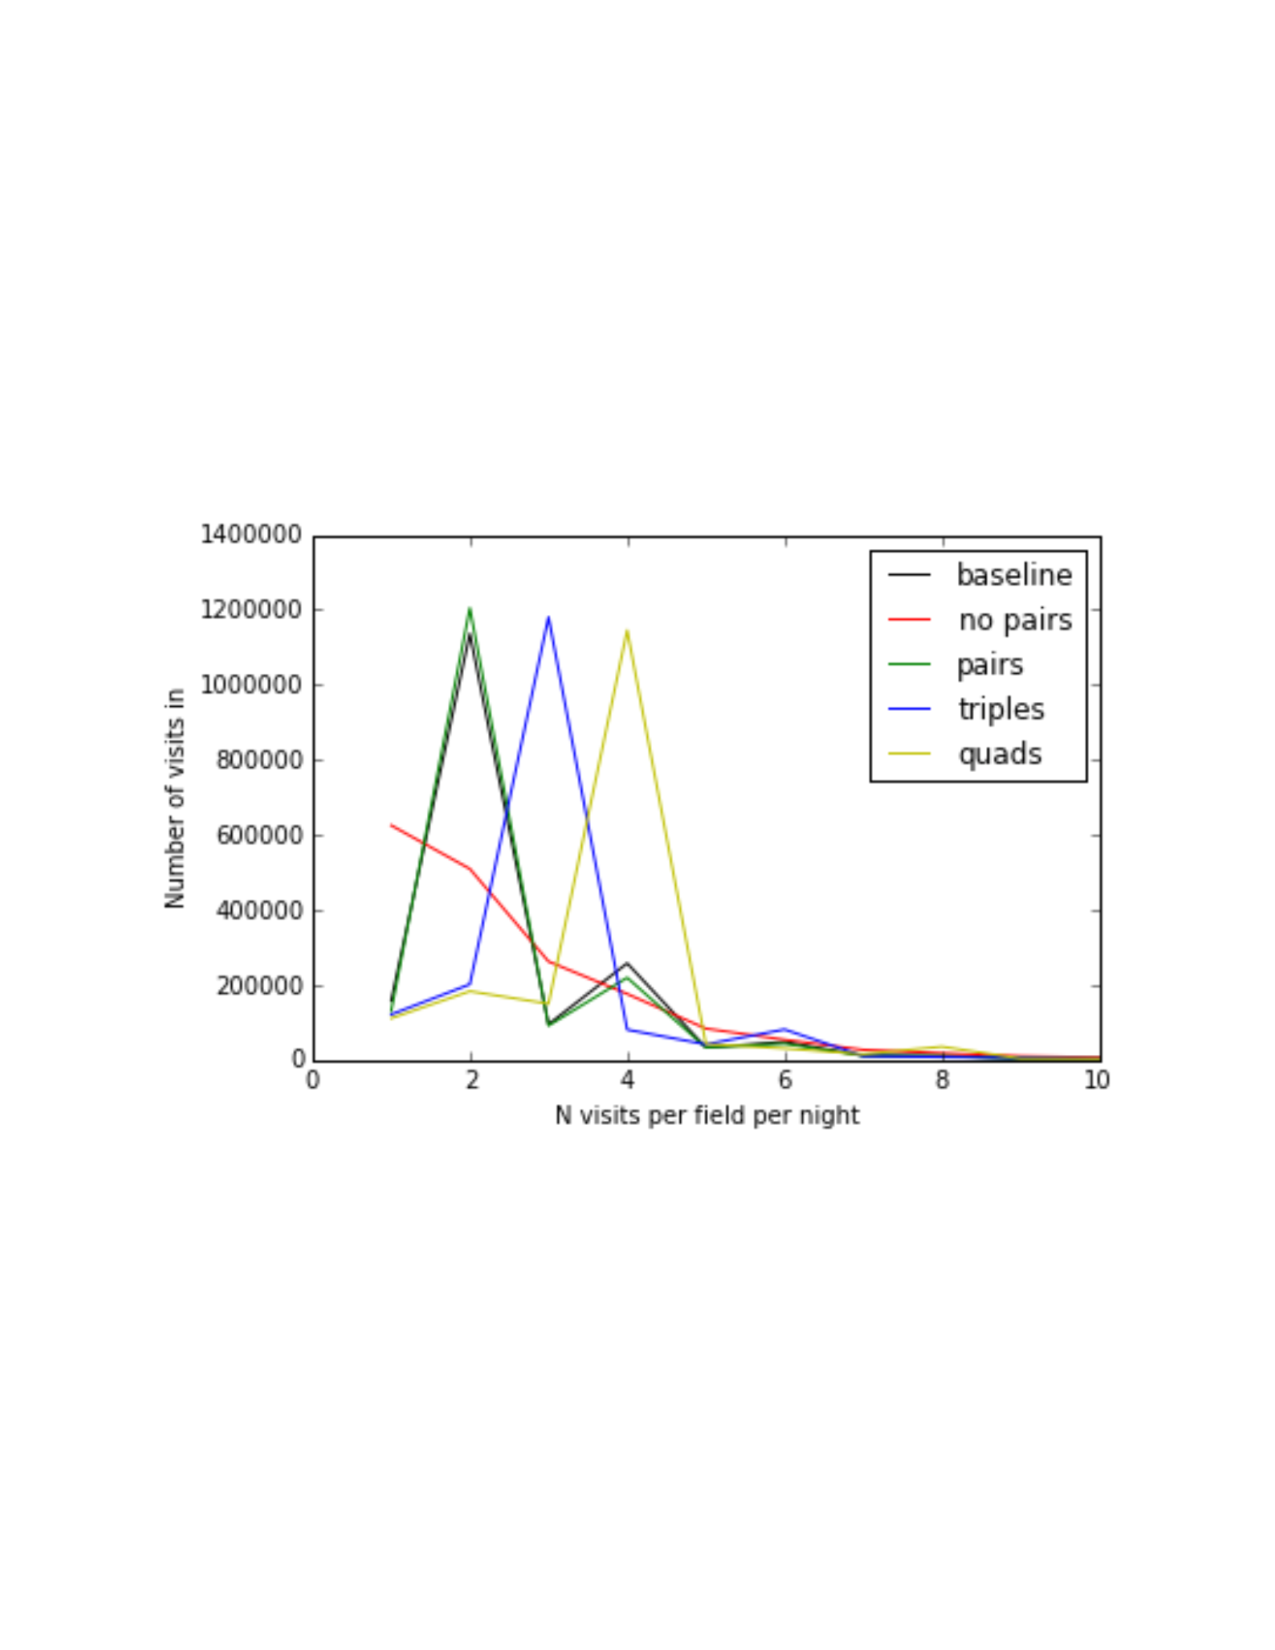
\includegraphics[angle=0,width=0.99\hsize:,clip]{figs/NvisitStats.pdf}
\vskip -2.7in
\caption{The distribution of the number of visits used for nightly sequences of
length given on the horizontal axis. Only $griz$ bands are used. Note that even
``no pairs'' simulation (\opsimdbref{db:NEOsNoVisitPairs})
includes multiple visits. The highest peak is at the
requested number of visits in a sequence.}
\label{fig:NvisitStats}
\end{figure}
%%%%%%%%%%%%%%%%%%%%%%%%%%%

%%%%%%%%%%%%%%%%%%%%%%%%%%%
\begin{figure}[t!]
\vskip -1.2in
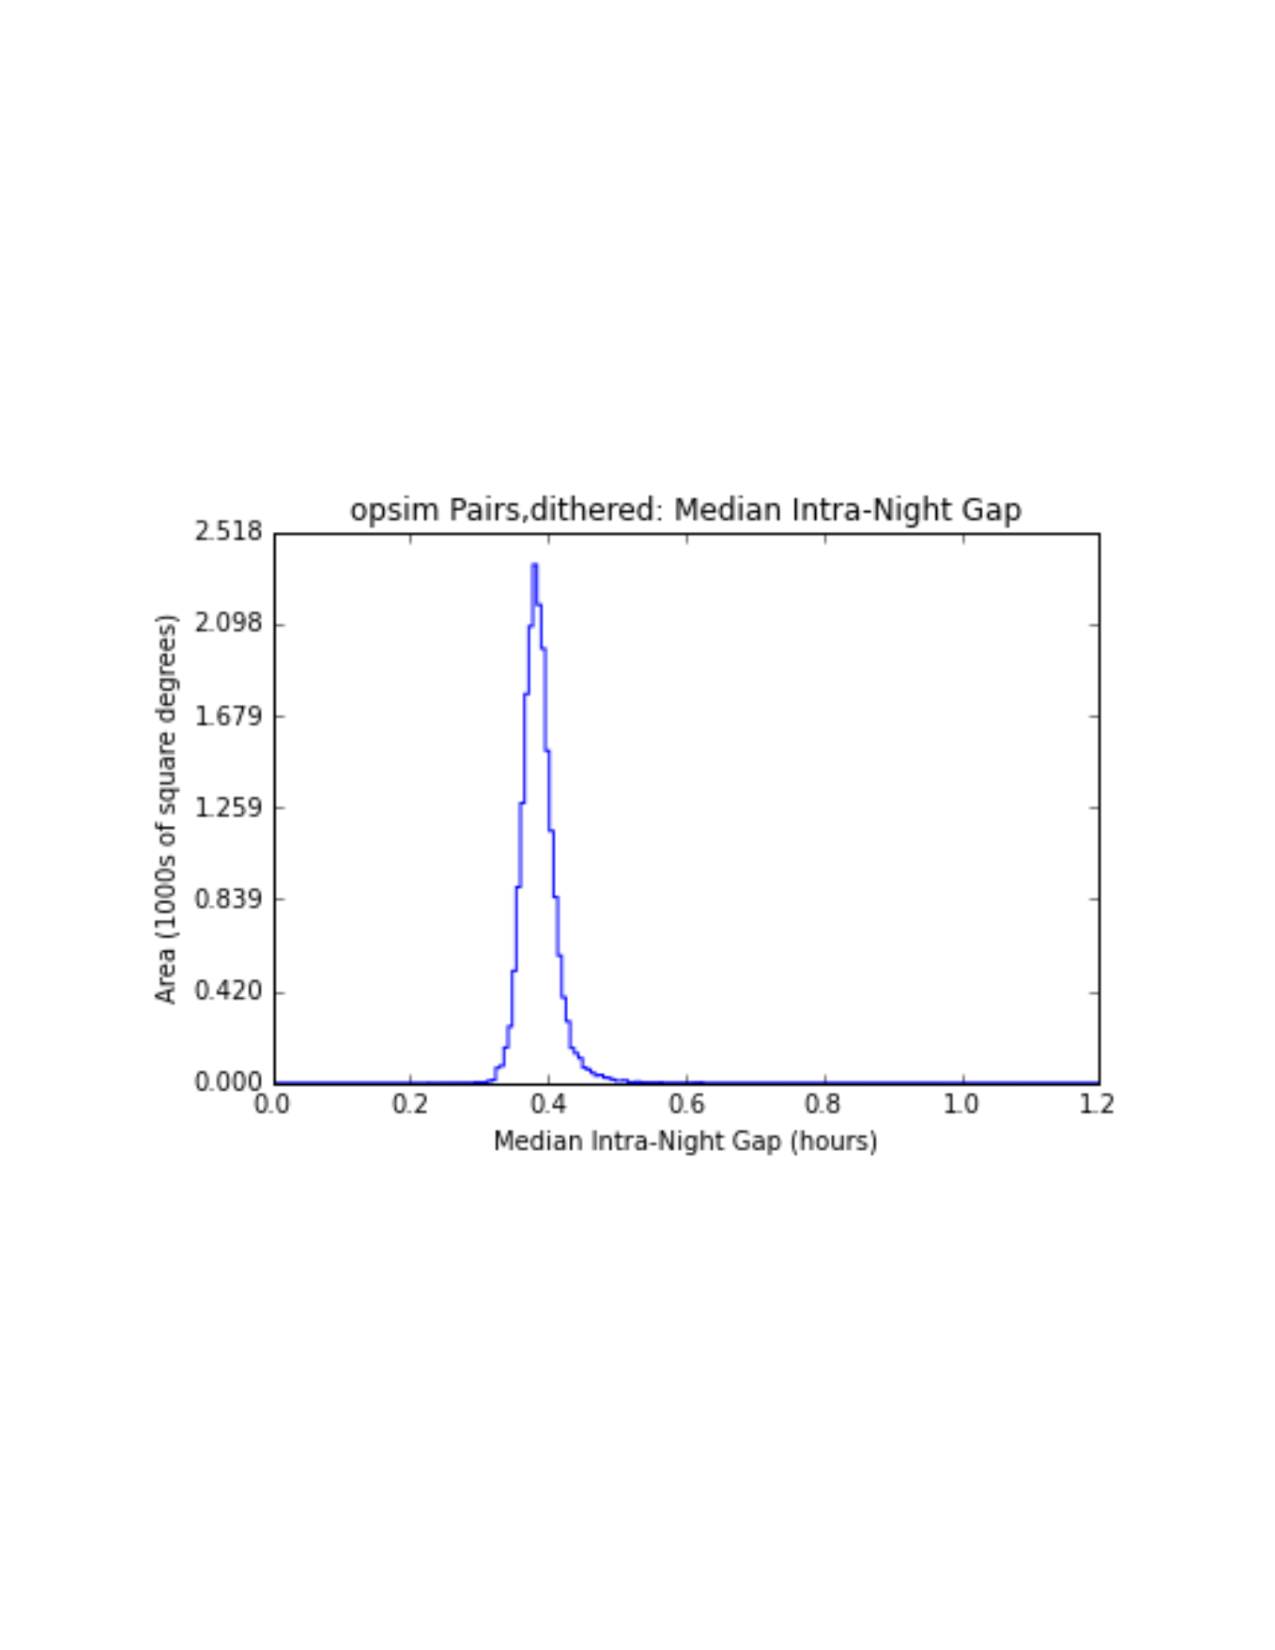
\includegraphics[angle=0,width=0.49\hsize:,clip]{figs/medinternight1.pdf}
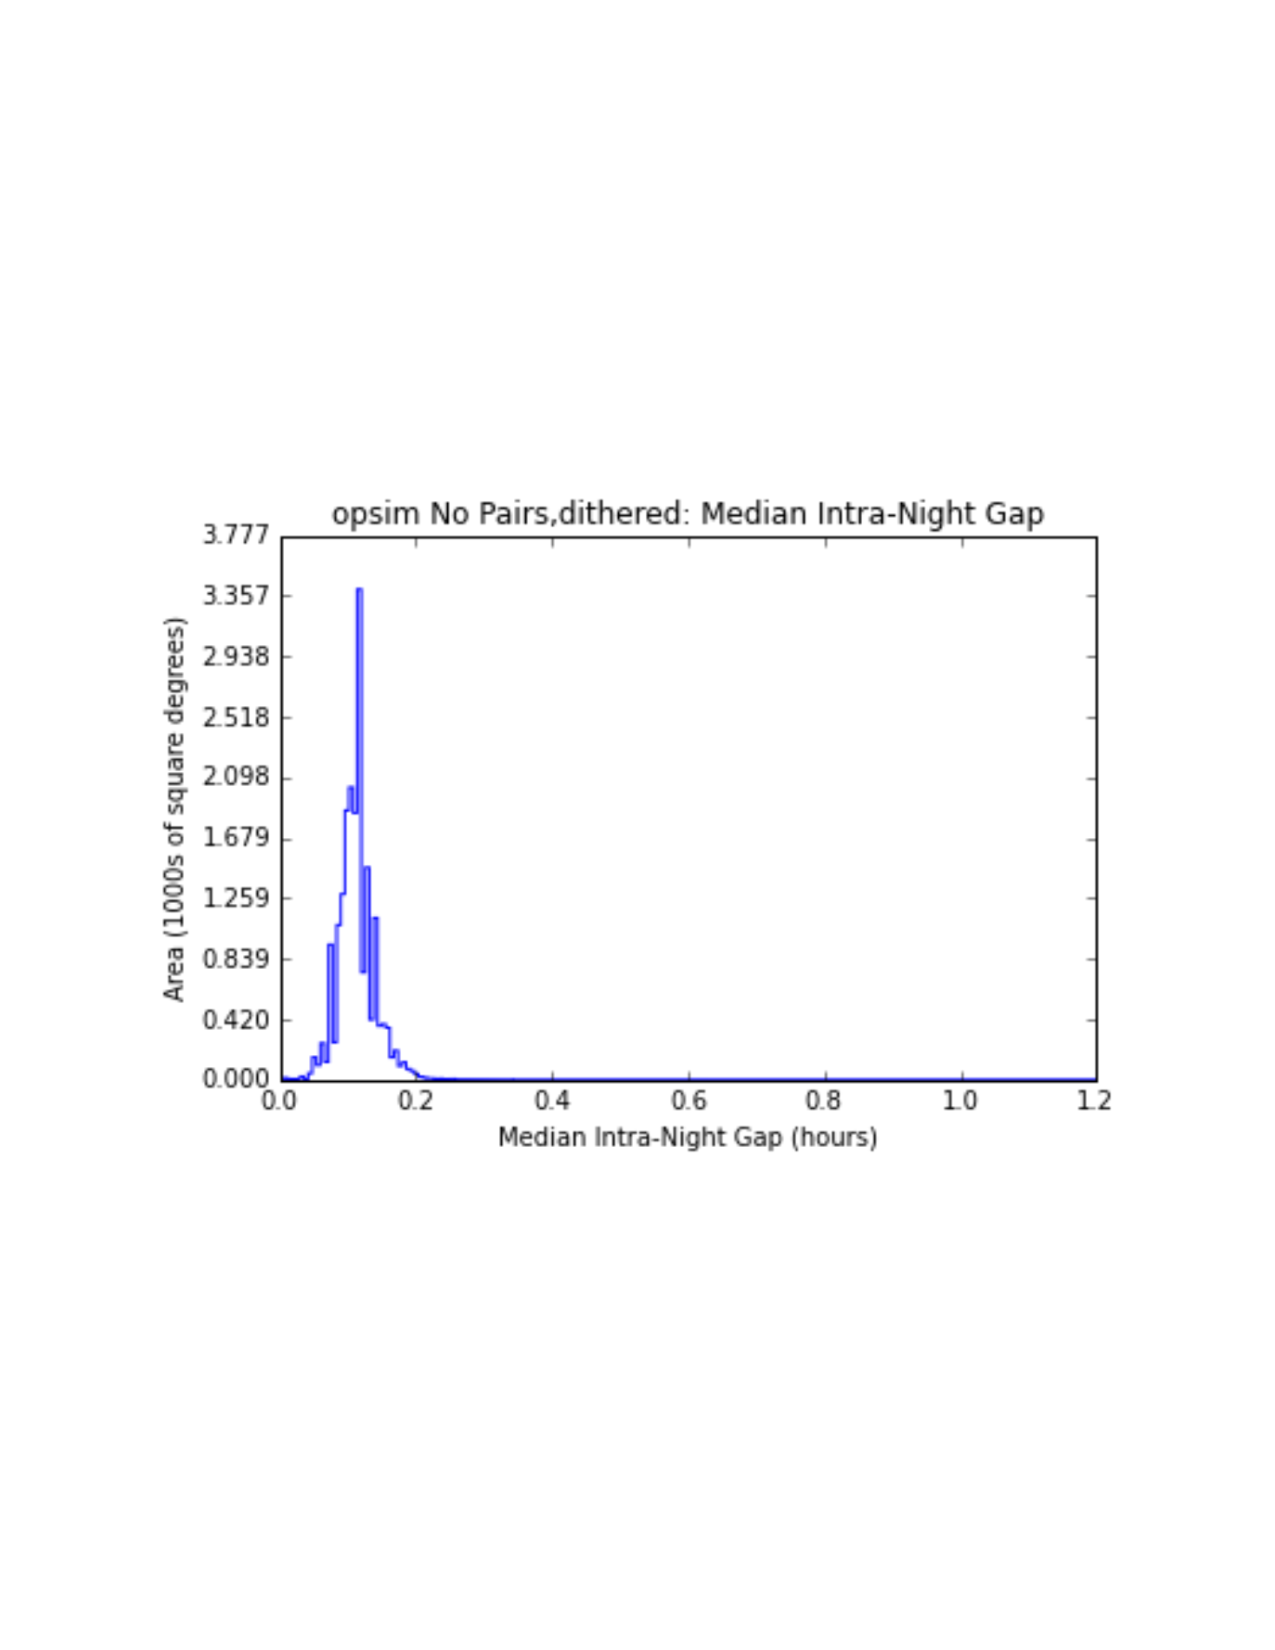
\includegraphics[angle=0,width=0.49\hsize:,clip]{figs/medinternight2.pdf}
\vskip -1.3in
\caption{
The comparison of the median intra-night gap distributions for Baseline Cadence (left)
and simulation \opsimdbref{db:NEOsNoVisitPairs}, which did not request pairs of visits per night.
Despite no need for pairs, simulation \opsimdbref{db:NEOsNoVisitPairs} produced them ``spontaneously'',
as well as longer sequences (see \autoref{fig:NvisitStats}). The mean field revisit
time is much shorter (about 6 minutes, see the right panel) than for Baseline Cadence
(22 minutes).}
\label{fig:intranightgapCompare}
\end{figure}
%%%%%%%%%%%%%%%%%%%%%%%%%%%

%%%%%%%%%%%%%%%%%%%%%%%%%%%
\begin{figure}[t!]
\vskip -1.1in
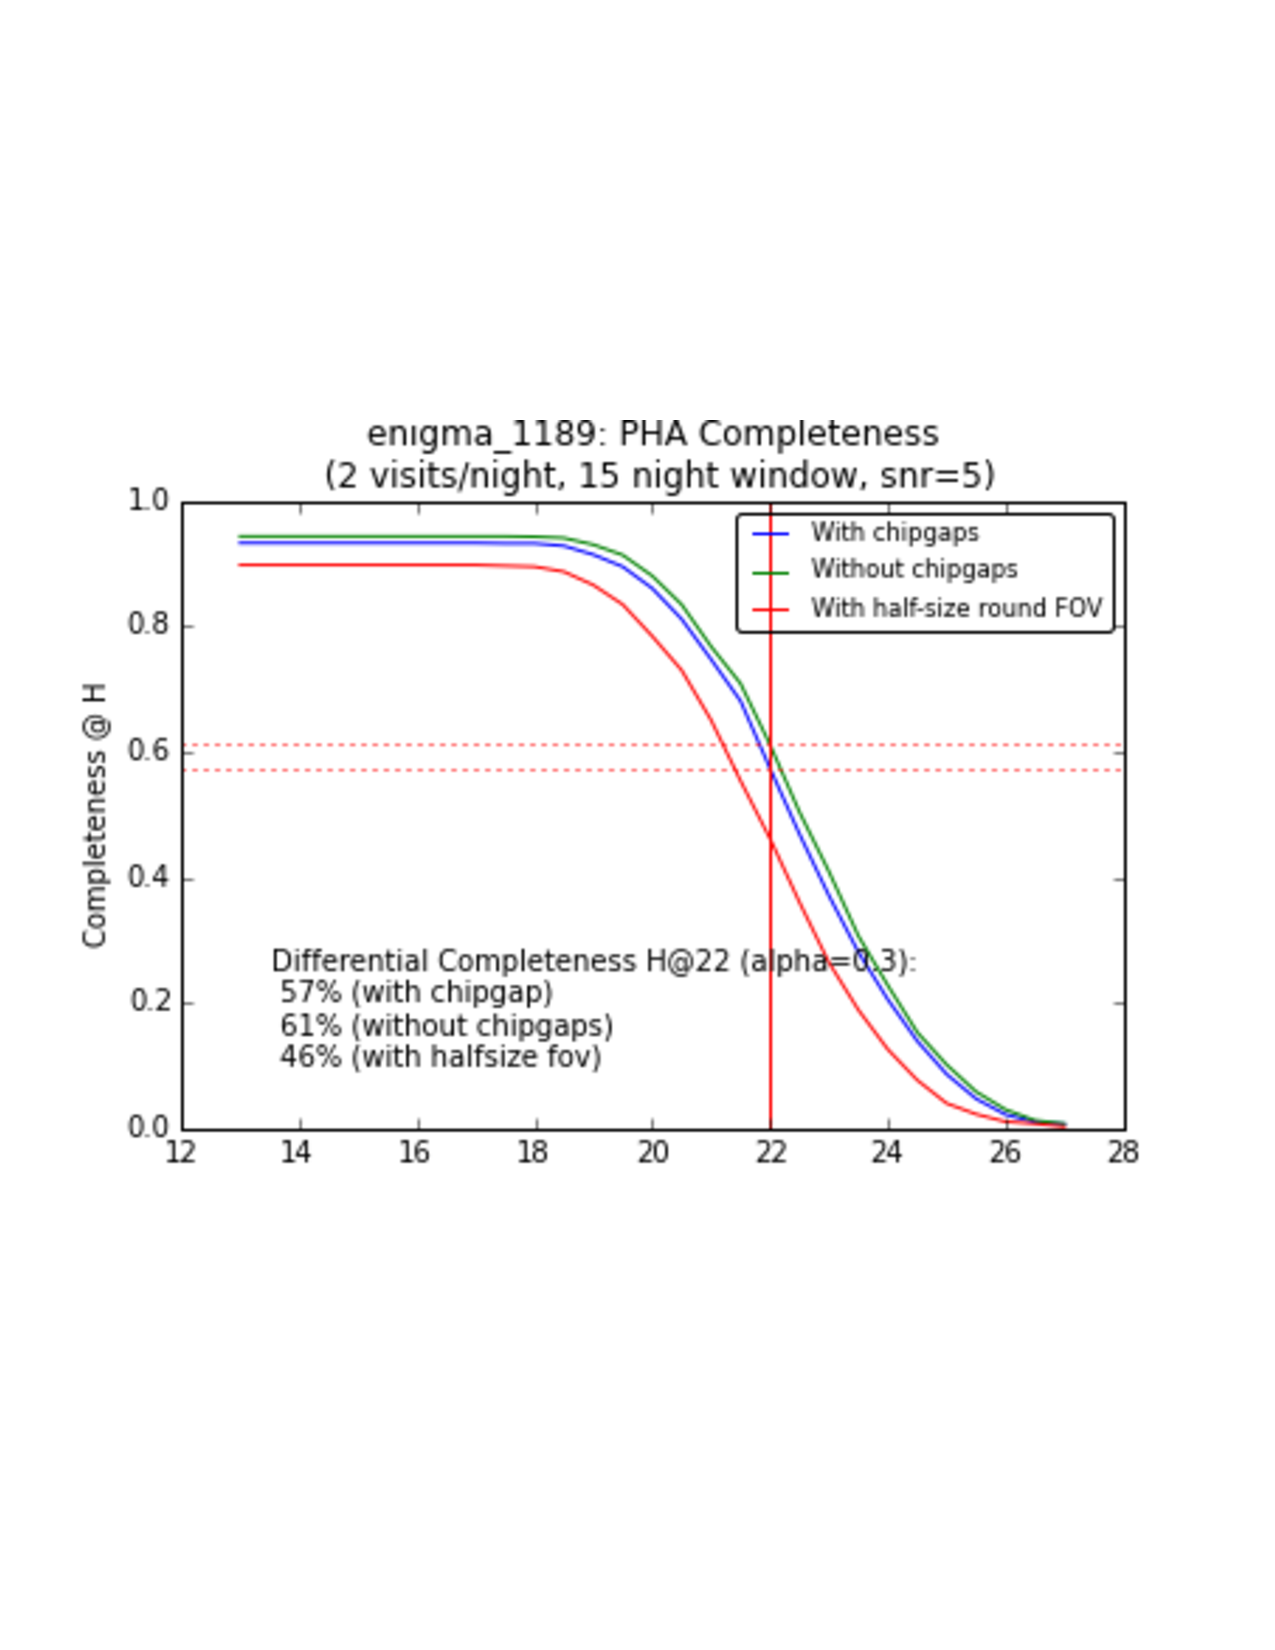
\includegraphics[angle=0,width=0.56\hsize:,clip]{figs/enigma1189_diffNEOcompleteness.pdf}
\hskip -0.5in
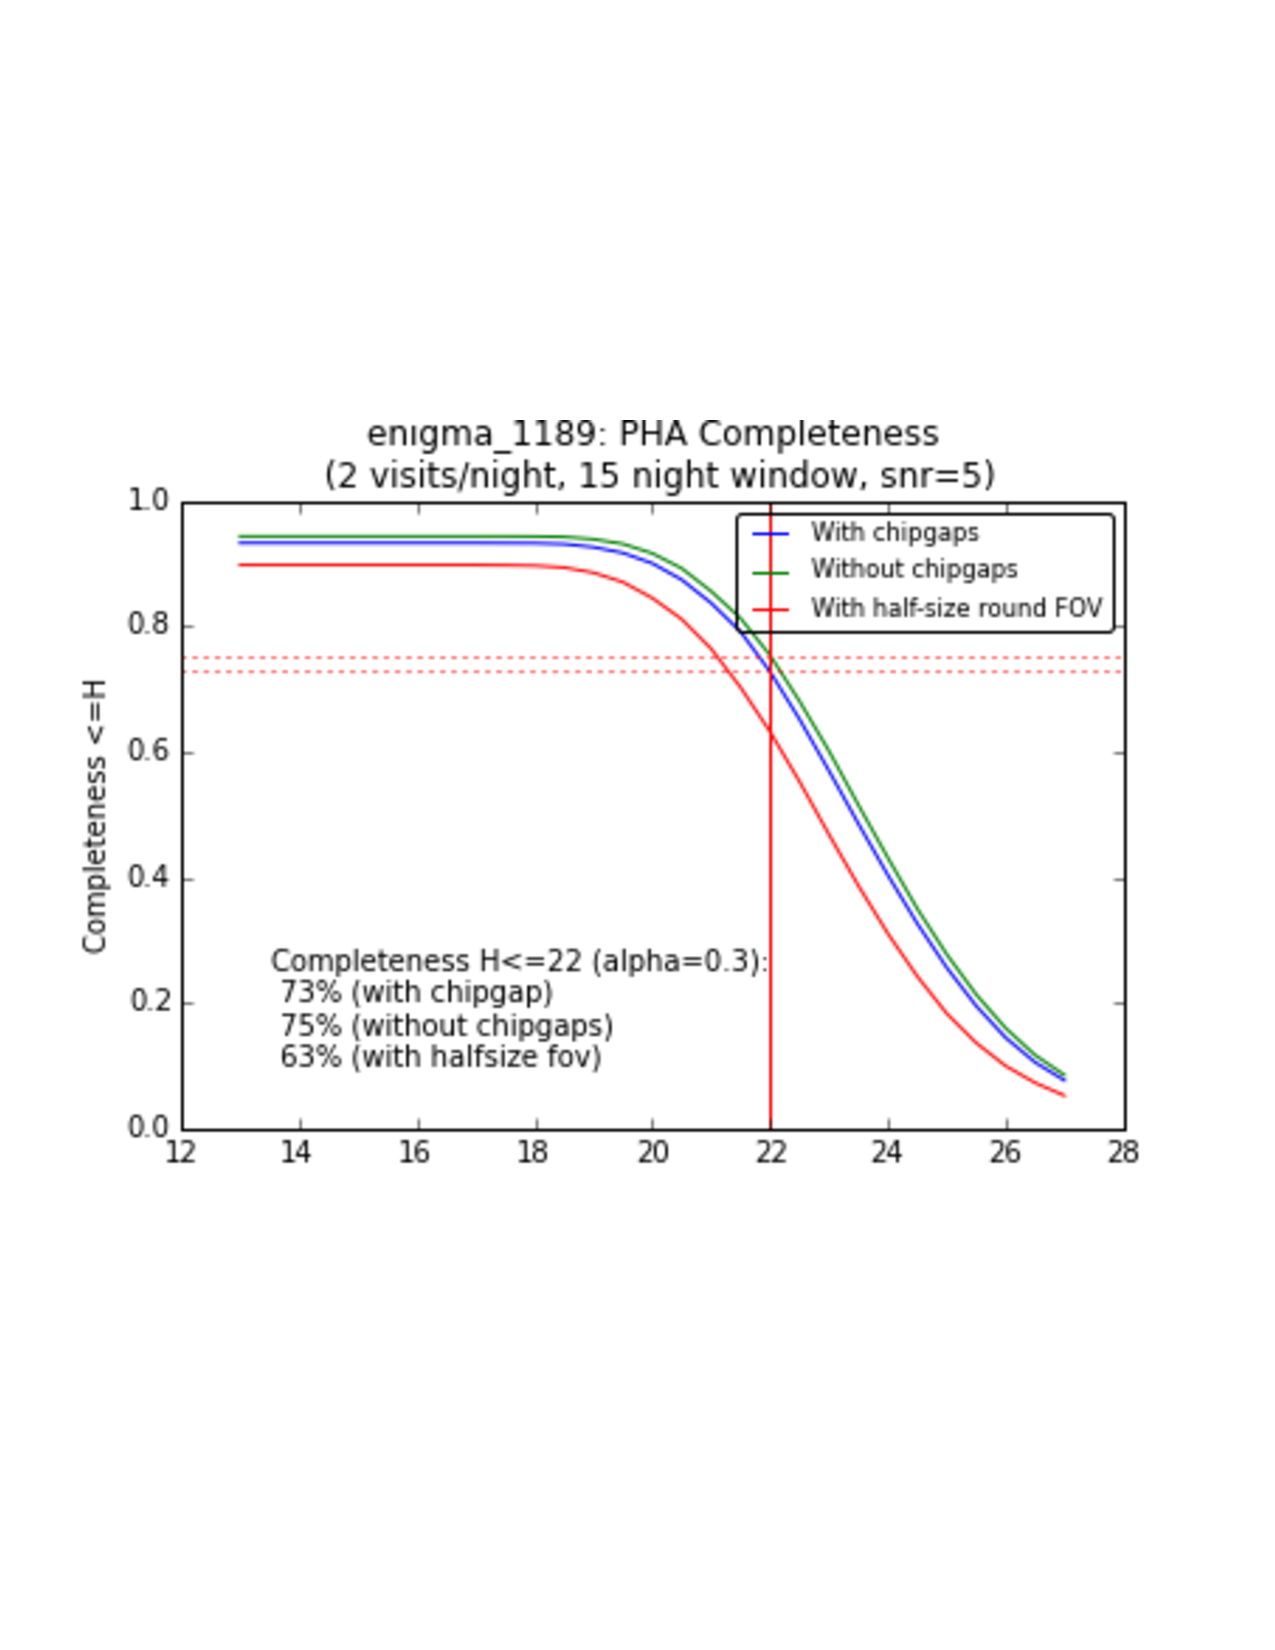
\includegraphics[angle=0,width=0.56\hsize:,clip]{figs/enigma1189_cumNEOcompleteness.pdf}
\vskip -1.2in
\caption{The PHA completeness for \opsimdbref{db:enigma}, as a function of the object's absolute
visual magnitude H on the horizontal axes (left: differential completeness at a given H;
right: cumulative completeness for all objects brighter than a given H).
The completeness for H$\le$22 NEOs (those with diameters larger than 140m)  for this
simulation is 73\% (blue line in the right panel). The panels also show the effects of ignoring
chip gaps (a 2\% effect for cumulative H$\le$22 completeness) and of decreasing the
field-of-view size to a half (i.e. to 4.8 sq. deg; a 10\% effect).}
\label{fig:enigmaNEO}
\end{figure}
%%%%%%%%%%%%%%%%%%%%%%%%%%%

%%%%%%%%%%%%%%%%%%%%%%%%%%%
\begin{figure}[th!]
\vskip -1.2in
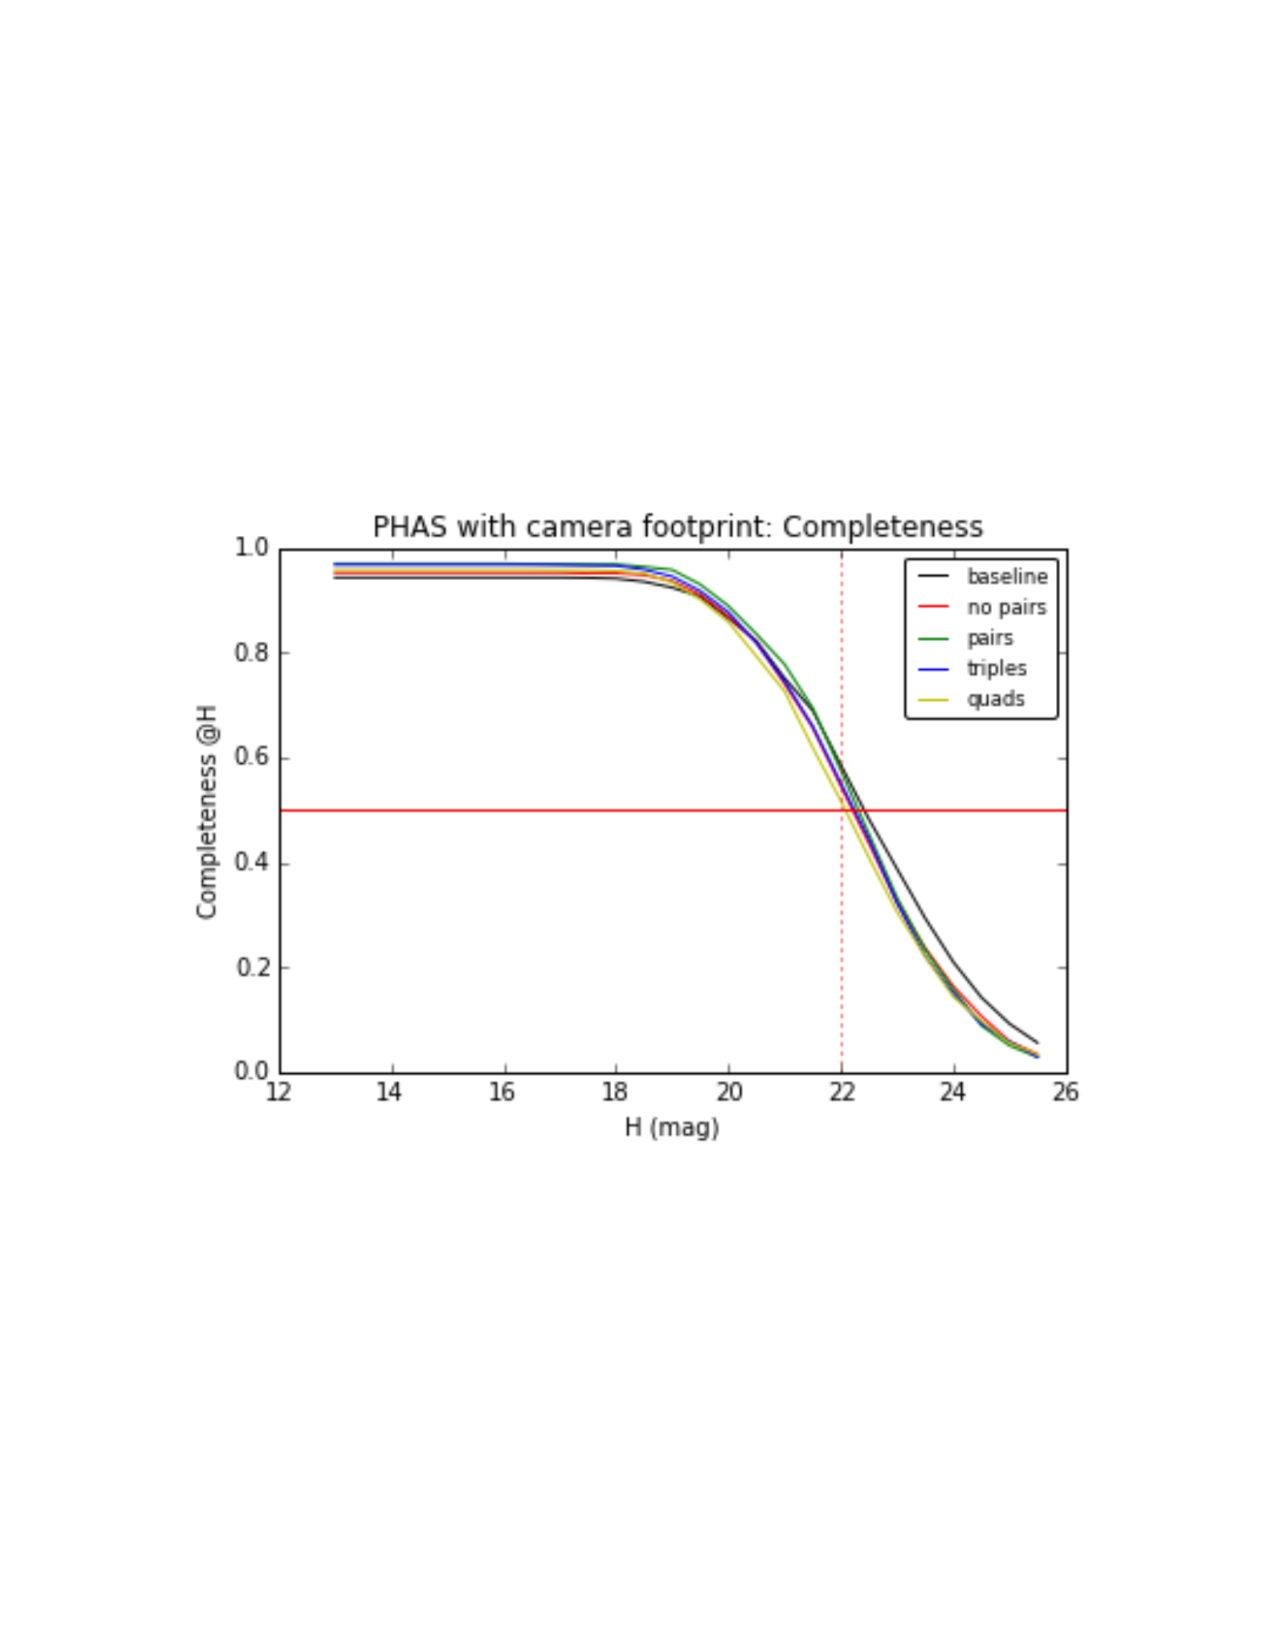
\includegraphics[angle=0,width=0.49\hsize:,clip]{figs/diffNEOpairs.pdf}
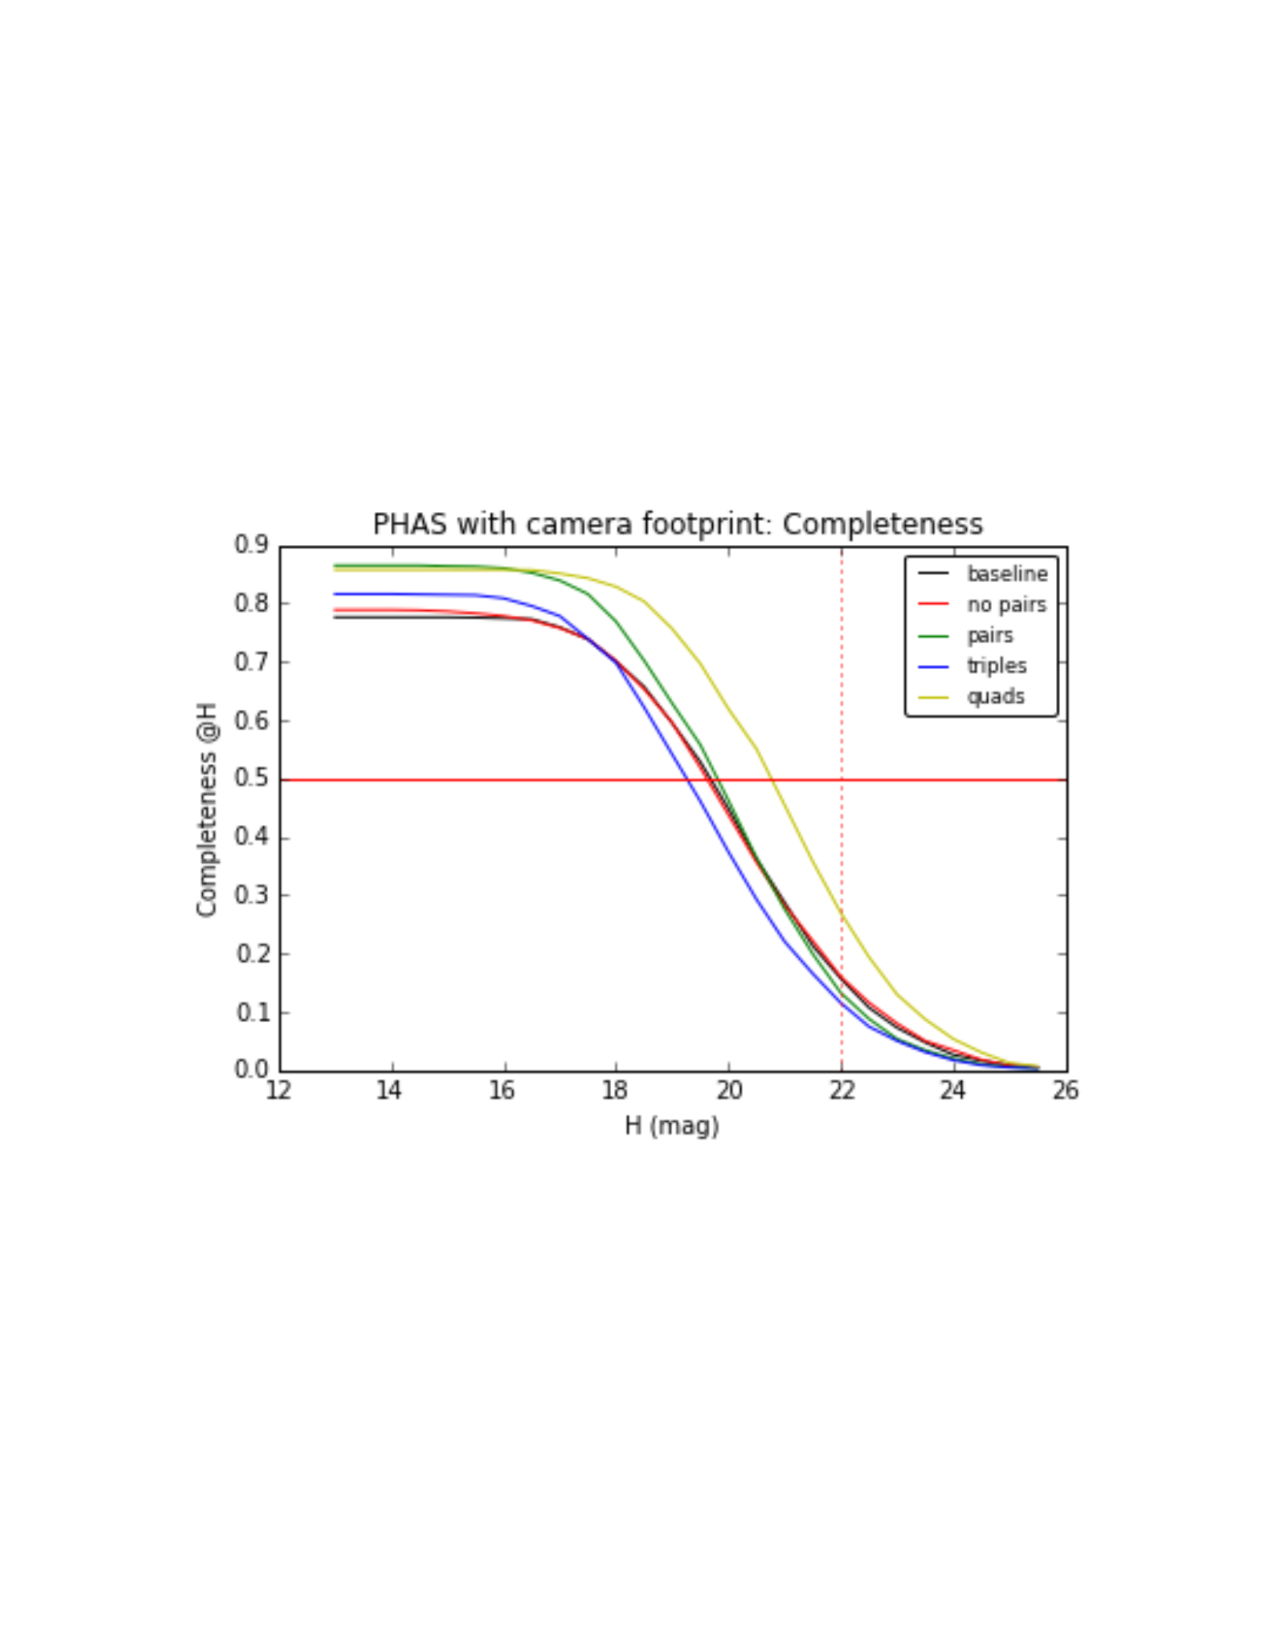
\includegraphics[angle=0,width=0.49\hsize:,clip]{figs/diffNEOquads.pdf}
\vskip -1.3in
\caption{
The comparison of differential PHA completeness for the five analyzed simulations
when requiring two detections per night (left) and four detections per night (right).
With two detections per night, all simulations perform similarly but when four
detections per night are required, the simulation that has the largest number
of such sequences (see \autoref{fig:NvisitStats}), performs the best although at an
inferior level compared to the left panel (see also \autoref{fig:enigmaNEO}).}
\label{fig:NEOquads}
\end{figure}
%%%%%%%%%%%%%%%%%%%%%%%%%%%


{\bf Analysis Results:}
First, we emphasize that ``requested'' is not the same as
``delivered'': even the ``no pairs''
simulation \opsimdbref{db:NEOsNoVisitPairs} ends
up having multiple visits in a given night to the same fields, and
when multiple visits per night are requested, not all fields get to
have completed sequences. The statistics of how many fields are
combined into sequences of a given number of visits is shown in
\autoref{fig:NvisitStats}.  As evident, the highest peak is at the
requested number of visits in a sequence, but not all visits are
incorporated into requested sequences: some are in both shorter and
longer sequences. In particular, even ``no pairs'' simulation includes
multiple visits to some fields, essentially because the current
version of the algorithm is not told not to do so. As illustrated in
\autoref{fig:intranightgapCompare}, such revisits typically happen
within 10 minutes from the first visit. This (unintended) behavior
implies that the naive expectation above is probably incorrect, as we
discuss in more detail below.


For baseline reference, the PHA completeness for
\opsimdbref{db:enigma} is shown in \autoref{fig:enigmaNEO}. The
baseline cadence achieves a cumulative completeness of 73\% for
H$\le$22 PHAs. This cumulative completeness for H$\le$22 is 17\%
higher than differential completeness at H=22 of 56\% due to
increasing completeness towards smaller H (larger objects). Both
differential and cumulative completeness are relevant metrics: the
former provides more insight in the behavior of a particular
simulation, while the latter is a metric given to NASA by the U.S.
Congress. Analysis of results illustrated in \autoref{fig:NEOquads}
can be summarized as follows:
\begin{itemize}
\item When NEO discovery algorithm requires pairs of visits, all runs
have very similar PHA completeness, with quads run only about 2\%
lower than the baseline (a differential completeness of 56\% at H=22
for \opsimdbref{db:enigma})
\item When NEO discovery algorithm requires 4 detections per night,
the simulation with quads achieves a differential completeness of
about 27\% at H=22, or  about 30\% lower completeness than Baseline
Cadence.
\item When NEO discovery algorithm requires 4 detections per night,
Baseline Cadence reaches a differential completeness of about 15\% at
H=22 (some quads are unintentionally produced by chance, see
\autoref{fig:NvisitStats}).
\item When NEO discovery algorithm requires 3 detections per night,
runs which requested triples and quads achieve a differential
completeness of about 40\% at H=22 (corresponding to a cumulative
completeness of about 57\% for H$\le$22).
\end{itemize}

Therefore, going from pairs of visits to triples (both for cadence and
NEO detection) reduces completeness (both differential and cumulative)
for PHAs with H$\le$22 by about 15-20\% (and by about 30\% for quads).


\subsubsection{Impact on other science programs}

The impact of requesting sequences with 3 or 4 visits to the same
field on other science programs is not yet analyzed in detail.  The
impact on static science should be minimal, except perhaps for a bit
worse behavior of various systematic errors (because fewer nights,
with their observing conditions, are sampled).

For time-domain science, the mean revisit time will increase by about
50\% if we go from pairs to triples, and by about a factor of two for
quads. This change will have a negative impact on time-domain science
programs based on SNe, variable stars, and transient objects, which
remains to be quantified.

\navigationbar

% --------------------------------------------------------------------

\section{Ongoing and Future Work}
\def\secname{cadexp:ongoing}\label{sec:\secname}


\subsection{Ongoing: Extended time-domain metrics}

A number of very sophisticated time-domain metrics have been
implemented in recent MAF development cycle (and some were contributed
by the community) but they have not been systematically run yet on all
available simulations. Time-domain metrics, together with metrics for
analyzing special programs (e.g. deep drilling programs), will be
further expanded in the next development cycle.


\subsection{Ongoing: Rolling Cadence experiments}

Analysis of a few prototype runs (\texttt{ops2\_1102},
\texttt{enigma\_1260}, \texttt{enigma\_1261}), which implemented the
so-called ``swiss cheese rolling cadence'' is in progress.


\subsection{Future work}

Based on analysis presented here, several recommendations
for further cadence exploration, can be made.

\begin{enumerate}

\item Further optimization of the main survey (e.g., exposure time in
general, and u band exposure time in particular; fixing western bias;
optimizing airmass limit and sky coverage; investigations of variable,
perhaps SNR-driven, exposure time).

\item Exploration and optimization of temporal sampling function in
general, and of Rolling Cadence in particular.

\item NEO completeness studies: what would it take for LSST to reach
90\% completeness for 140m and larger NEOs?  Based on previous
analysis, directions to explore are deeper visits along the Ecliptic
and longer survey duration (about 12 years).

\item Exploration of extending the main survey to the Galactic plane
(per A. Gould's proposal, arXiv:1304.3455) and further optimization of
Galactic plane and Bulge science programs.

\item Optimization of LMC/SMC coverage (and somewhat less importantly,
the South Celestial Pole coverage).

\item Deep drilling optimization (detailed analysis of existing
proposals; investigation of gains from going to a larger observing
time allocation, e.g. 20\%).

\item Twilight short-exposure time observing (per internal Stubbs proposal).

\item Planning commissioning observations (e.g. the tension between
going wide to enable self-calibration and dense temporal sampling to
obtain various light curve templates and fine tune image differencing
and multi-epoch data processing and data analysis software tools).

\item Dynamic cadence explorations (the main goal at this time is to
answer: are our tools good enough to act and react swiftly and
robustly in operations?).

\end{enumerate}

\navigationbar

% --------------------------------------------------------------------

\section{Summary}
\def\secname{cadexp:summary}\label{sec:\secname}

The most important conclusion of this study is that the upper limit on
possible scheduling efficiency improvements for Baseline Cadence is
close to 6\%. This conclusion is by and large based on the fact that
the mean slew time for (candidate) Baseline Cadence is 6.9 sec, and
thus only slightly larger than the design specifications for the
system slew and settle time of 4.5 sec.  Nevetheless, there are a
number of features to understand, and some to fix, and there is
substantial optimization potential in temporal sampling functions and
further optimization of the sky area and observing strategy details,
that can result in enhanced science even with the same integrated
open-shutter time (e.g. by obtaining deeper data through an improved
sampling of observing conditions).

\vskip 0.2in
The main other questions addressed here are:

\begin{enumerate}

\item {\it By what factor could we exceed the SRD design specification
for the number of visits if only Universal Cadence proposal was
implemented?}

A simulation that only implemented Universal Cadence proposal exceeded
the design specification for the number of visits by about 40\% (over
the design specification for the sky area of 18,000 sq.deg.)

\item {\it By what factor could we exceed the SRD design specification
for the sky coverage if only Universal Cadence proposal was
implemented with the design specification for the number of visits?}

This Pan-STARRS-like strategy results in about 40\% larger sky
coverage (about 25,000 sq.deg.), with the mean number of visits at
92\% of the design specification. The total number of visits is the
same as for Baseline Cadence, implying similar surveying efficiency.

Therefore, the available ``margin'' relative to the SRD design specifications
for the main survey is equivalent to about 30-40\% larger sky coverage, or
about 30-40\% more visits per field. The SRD assumes that 10\% margin
will be available for other programs. The implied ``survey reserve'',
relative to the Universal Cadence design specifications from the SRD, can
be used to:
  \begin{enumerate}
  \item increase the number of visits per field over the WFD area,  or
  \item increase the surveyed area while keeping the number of visits
  per field statistically unchanged, or
  \item increase both area and the number of visits, and/or
  \item execute additional programs (the current baseline).
  \end{enumerate}

\item {\it What is the effect of auxiliary proposals on surveying
efficiency?}

A comparison of simulations which only implemented Universal Cadence
proposal to those that included all other programs did not show a
significant change of efficiency (older simulations, not analyzed
here, showed increases in surveying efficiency of up to about 3\% due
to shorter slewing time).


\item {\it What is the effect of visit pairs on surveying efficiency? }

Relinquishing the visit pair requirement results in up to 2-3\%
improvement of the surveying efficiency. The impact on some
time-domain science would be positive, while for NEO and main-belt
asteroid science it would be strongly negative.


\item {\it Can the effects of variations of the visit exposure time on
surveying efficiency be predicted using simple efficiency estimates?}

Simple estimates based on comparing exposure (open shutter) and total
visit times are in good agreement with simulations. Decreasing the
visit exposure time to 20 seconds decreases the total open shutter
time by 10\%, and increasing it to 60 seconds increases the total open
shutter time by 16\%, relative to Baseline Cadence and standard
exposure time of 30 seconds. The number of visits changes by factors
of 1.35 and 0.58.


\item {\it What are the effects of doubling the exposure time only in
the $u$ band?}

The effect of doubling the exposure time only in the $u$ band, while
simultaneously halving the number of requested visits, has no
significant effect on the survey efficiency.

The effect of doubling the exposure time only in the $u$ band, with
the number of requested visits unchanged, is a decrease in the number
of visits in other bands by about 6\%.


\item {\it What is the impact of hard airmass limit, $X<1.5$, on the
surveying efficiency?}

It is a very bad idea to relax airmass limit! It is possible to
achieve the same surveying efficiency with much more stringent airmass
limit than 1.5, which was used in most simulations to date.

\end{enumerate}


\navigationbar
